\documentclass[a4paper, 12pt]{article}
\usepackage{config}

\begin{document}
	\begin{center}
		\begin{huge}
			Resumo dos Comandos
		\end{huge}
	\end{center}

	\begin{itemize}
		\item Lista de comandos a ser tratada
		\begin{itemize}
			\item\ttt{Plot}
			\item\ttt{Plot3D}
			\item\ttt{ContourPlot}
			\item\ttt{ContourPlot3D}
			\item\ttt{ParametricPlot}
			\item\ttt{ParametricPlot3D}
			\item\ttt{StreamPlot}
			\item\ttt{VectorPlot}
			\item\ttt{Show}
		\end{itemize}
	\end{itemize}

	\section{Plot}
	Normalmente recebe uma função que depende de somente uma variável seguida da definição do intervalo de amostragem desejado. Então imagine que se deseja plotar a função do segundo grau $f(x)=x^{2}$, para fazer isso basta tomar o lado direito da função e utilizar como primeiro parâmetro do \ttt{Plot} como segue.	

\begin{lstlisting}[language=Mathematica]
Plot[x^2]
\end{lstlisting}
	
	Porém, não é adequado parar por aqui, é necessário definir a variação de $x$ em uma dimensão que vai abranger o ``teatro'' escolhido. Dessa maneira, imagine que queiramos plotar essa função de modo a abranger os valores de $x$ que vão de -1 a 1, então aplicamos \ttt{\{x,-1,1\}}. Como consequência, percebe-se que o programa lança valores de $x$ abrangendo o domínio explicitado de modo a conformar a representação gráfica no menor espaço possível de visualização para os valores de $x$ escolhidos
	
\begin{lstlisting}[language=Mathematica]
Plot[x^2,{x,-1,1}]
\end{lstlisting}

	Da forma como está, se dermos \ttt{<enter>} o comando será rodado e vamos obter
	
	\begin{figure}[!h]\label{parabola}
		\centering
		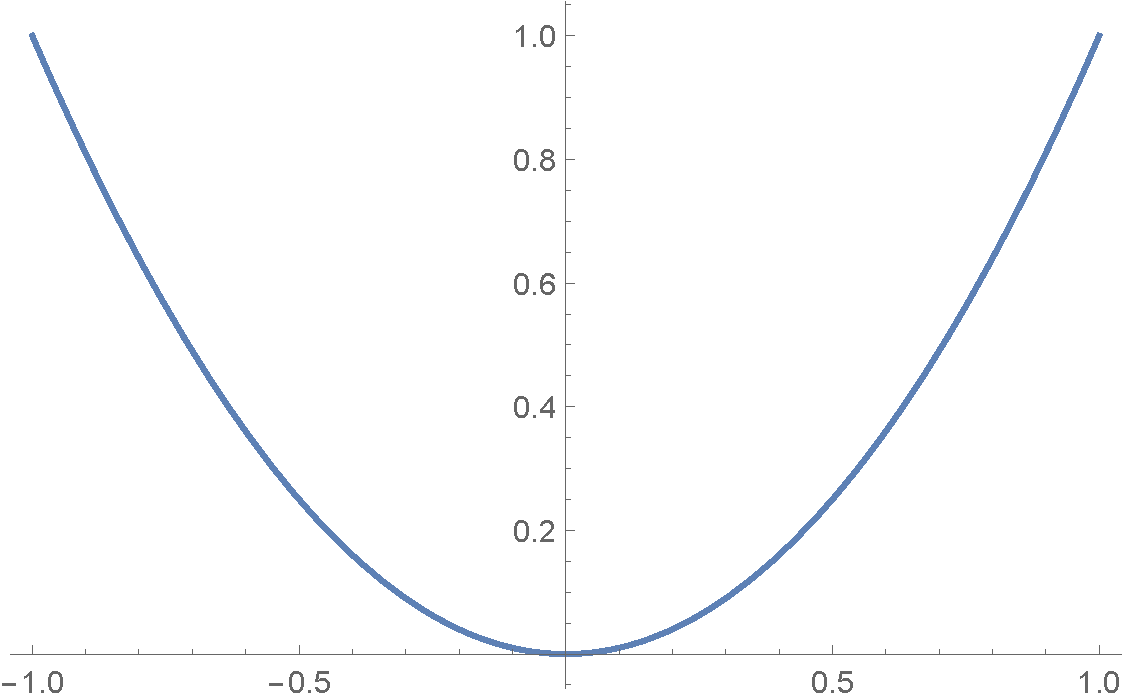
\includegraphics[scale=.5]{images/parabola}
	\end{figure}

	Repare que sendo $x=-1$ ou $x=1$, $f(x)=1$, logo o máximo valor de $f$ mostrado é 1, não precisamos da variação de $y$, até mesmo por que o \ttt{Plot} não aceitaria tal sintaxe. Ele apenas subentende que os valores de $y$ que darão as dimensões ao lugar do gráfico são provenientes da substituição de $x$ em $f$.
	
	\section{Plot3D}
	Podemos interpretar esse comando como expansão do \ttt{Plot}, porém em três dimensões. Sabendo que um ponto no espaço agora depende de $x$ e $y$, consequentemente a função $f(x)$ em duas dimensões passará a ser $f(x,y)$. De forma análoga ao que foi feito para o comando anterior, imagine que queiramos plotar um paraboloide no espaço que obedeça a função
	
	\begin{equation}
		f(x,y)=x^2+y^2
	\end{equation}
	
	Numa abordagem rápida, pode-se imaginar tal superfície como a rotação de uma parábola tal como é visto em \ref{parabola} ao redor do eixo $z$ no espaço, então sabendo que dependemos de mais uma variável será preciso acrescentar outro parâmetro ao \ttt{Plot3D} como segue
	
\begin{lstlisting}[language=Mathematica]
Plot3D[x^2+y^2,{x,-1,1},{y,-1,1}]
\end{lstlisting}
	
	\begin{figure}[!h]
		\centering
		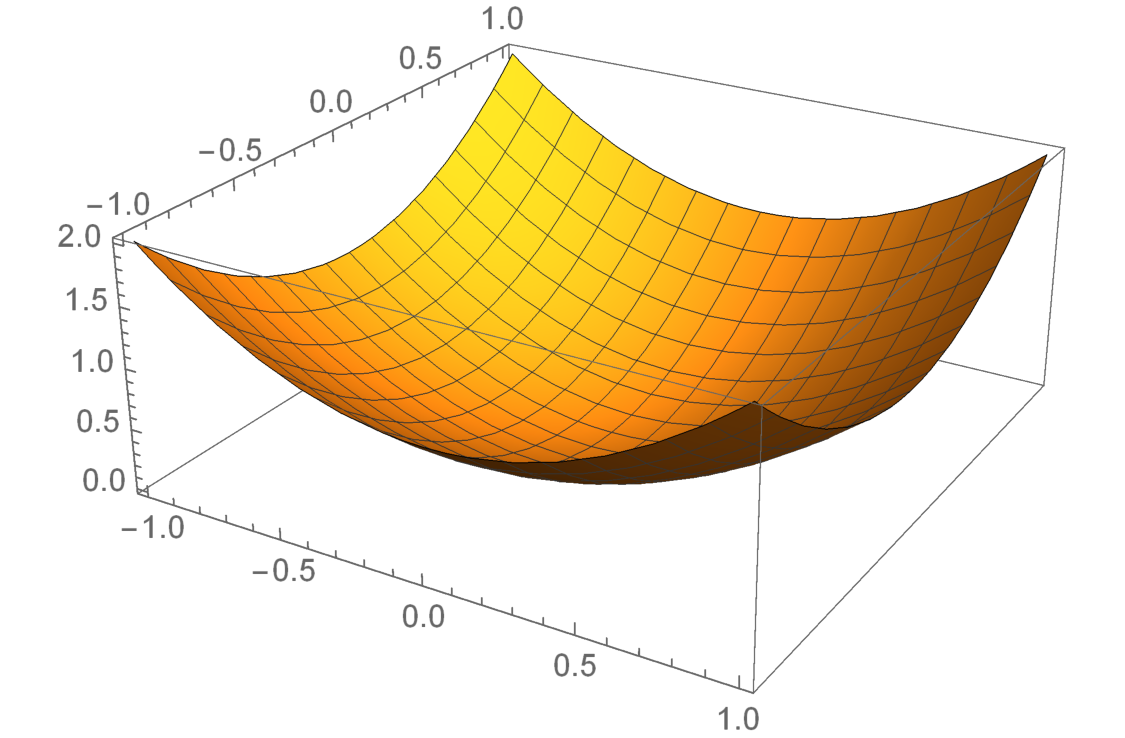
\includegraphics[scale=.6]{images/parabola3d}
	\end{figure}

	Note que se clicarmos com o botão direito do \textit{mouse} e formos na opção \textit{Top View} veremos
	
	\begin{figure}[!h]
		\centering
		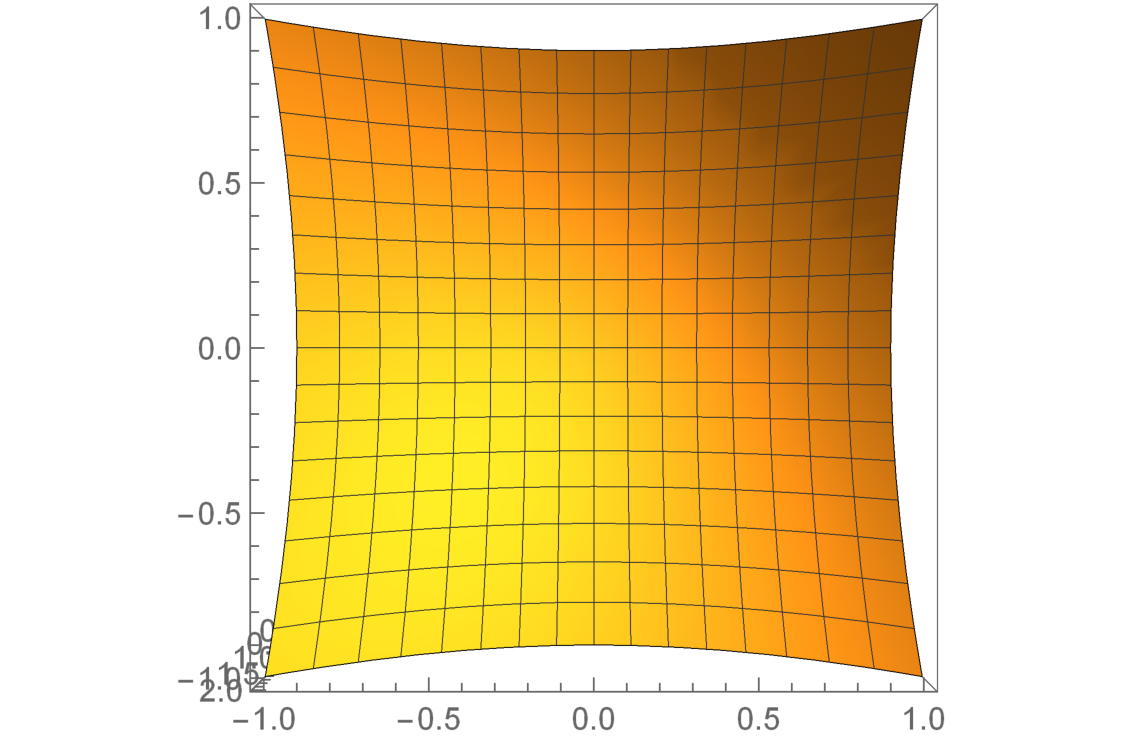
\includegraphics[scale=.55]{images/parabola3dtop}
	\end{figure}
	
	Ou seja, o intervalo de valores escolhido para $x$ e $y$ novamente é notado no domínio. Vê-se que a vista superior é um quadrado de lado valendo 2 unidades. Isso ocorre pois tanto $x$ quanto $y$ variam entre menos -1 e 1.
	
	Partindo para análise em $z$, vamos mudar a opção de \textit{Top View} para \textit{Front View}. Ao visualizar, nota-se que a máxima altura da ``caixa'' que comporta o gráfico é de duas unidades. Tal fenômeno é decorrente do máximo valor que $f(x,y)$ pode assumir para o domínio escolhido que, nesse caso, é quando as coordenadas são $(-1,-1)$, $(-1,1)$, $(1,-1)$ ou $(1,1)$ como vemos a seguir
	
	\begin{figure}[!h]
		\centering
		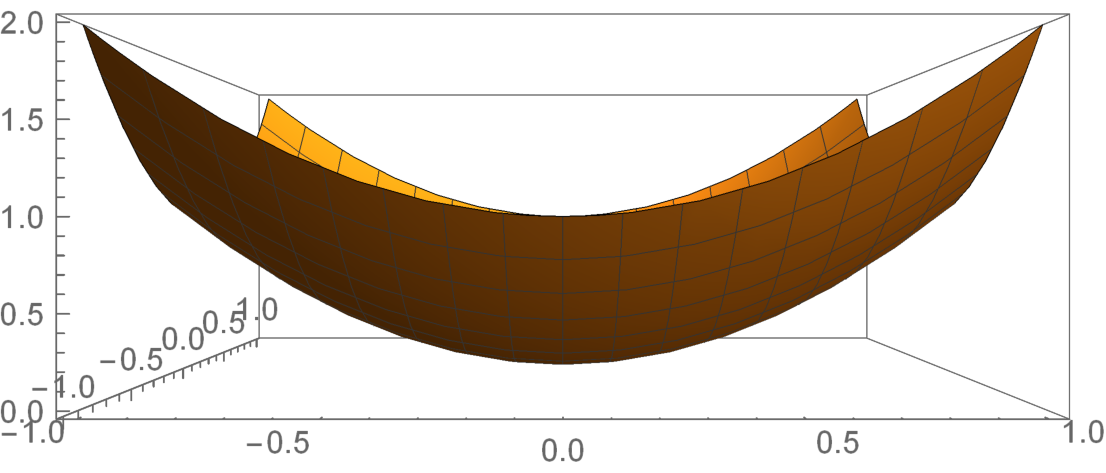
\includegraphics[scale=.55]{images/parabola3dfront}
	\end{figure}

	Sabemos disso devido a simplicidade do gráfico e prevemos que a função é sempre crescente no intervalo dado.
	
	Alguns atributos de estilo podem ser passados para os \ttt{Plot}s de modo a melhorar a visualização ou visando cumprir alguma meta de representação gráfica. Alguns dos comandos a seguir são interessantes de serem entendidos pelo menos no básico.
	
	\vspace{.5cm}
	Para o \ttt{Plot} (Gráficos em 2d no geral) 
	\begin{itemize}
		\item\ttt{AspectRatio}
		\begin{itemize}
		\item Permite editar a proporção entre os eixos do gráfico. Imagine que quiséssemos uma proporção de 1 em $x$ para dois em $y$, teríamos uma razão igual a 0.5 e podemos prever que o gráfico terá maior comprimento em $x$ que em $y$ como vemos a seguir com base nas linhas de comando
		\end{itemize}
	
\begin{lstlisting}[language=Mathematica]
Plot[x^2,{x,-1,1},AspectRatio->.5]
\end{lstlisting}
		
		\begin{figure}[!h]
			\centering
			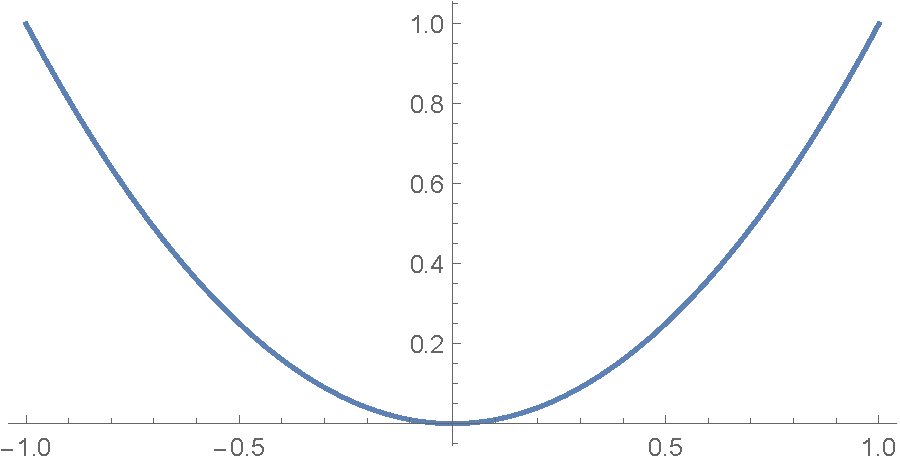
\includegraphics[scale=.55]{images/aspecthalf}
		\end{figure}
		
		Trocando por 2 o valor da propriedade vemos
		
\begin{lstlisting}[language=Mathematica]
Plot[x^2,{x,-1,1},AspectRatio->2]
\end{lstlisting}
		
		\newpage 
		\begin{figure}[!h]
			\centering
			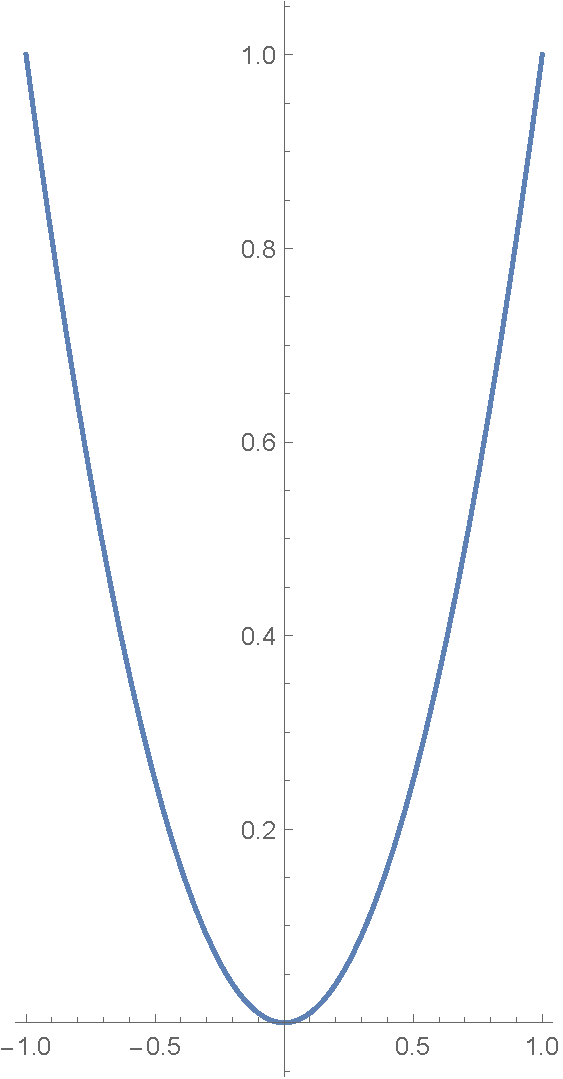
\includegraphics[scale=.55]{images/aspectdouble}
		\end{figure}
	
		\item\ttt{PlotStyle} 
			\begin{itemize}
				\item Um dos atributos mais utilizados, possibilita mudar a cor do gráfico, espessura das linhas, opacidade, entre muitos outros parâmetros. 
				\begin{itemize}
					\item Mudando a cor
					\begin{itemize}
						\item Uma maneira aconselhável é passar diretamente o atributo de cor empregando, por exemplo: \ttt{Magenta}, \ttt{Red}, \ttt{Blue}, \ttt{Cyan} ou utilizar o \ttt{RGBColor} para customizar com maior liberdade como segue
					\end{itemize}
				\end{itemize}
			\end{itemize}
		
\begin{lstlisting}[language=Mathematica]
Plot[x^2,{x,-1,1},AspectRatio->.5,PlotStyle->Magenta]
\end{lstlisting}

\begin{figure}[!h]
	\centering
	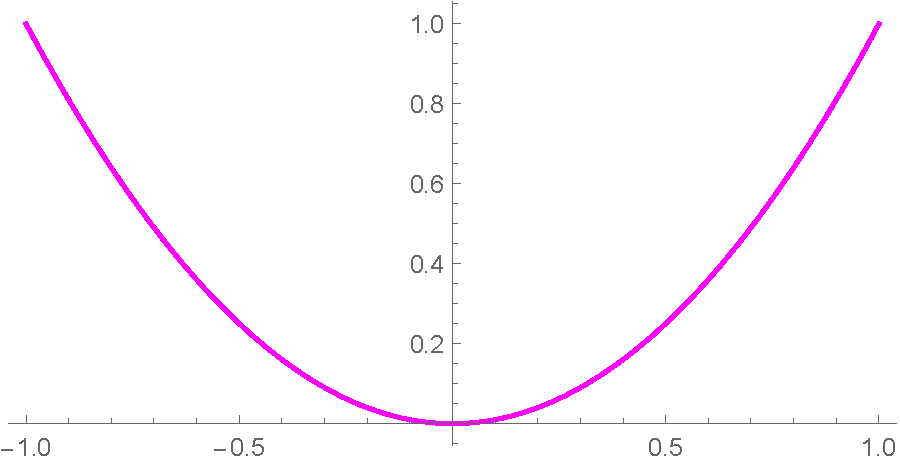
\includegraphics[scale=.55]{images/magenta}
\end{figure}

		\item\ttt{GridLines} 
		\begin{itemize}
			\item Nos permite adicionar uma malha quadriculada ao fundo da plotagem. Esse recurso muitas vezes facilita a associação entre os eixos coordenados e nos permite ter maior precisão quantitativa para aproximações feitas visualmente. Abaixo temos alguns exemplos.
		\end{itemize}


\begin{lstlisting}[language=Mathematica]
Plot[x^2,{x,-1,1},AspectRatio->.5,PlotStyle->Magenta,GridLines->Automatic]
\end{lstlisting}
\begin{figure}[!h]
	\centering
	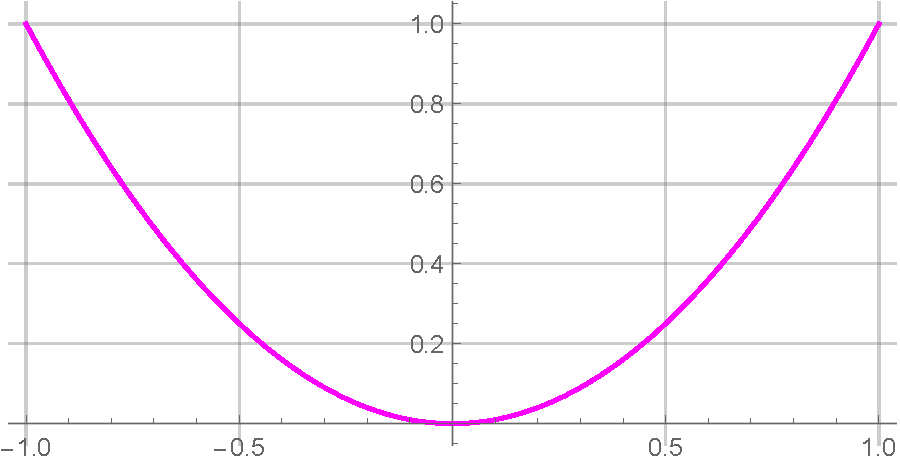
\includegraphics[scale=.55]{images/grid}
\end{figure}
		
		\begin{itemize}
			\item[] Por padrão o \ttt{GridLines} com \ttt{Automatic} renderiza linhas cheias, mas podemos alterá-las passando \ttt{GridLinesStyle->\{\{Dashed\},\{Dashed\}\}}. Isso fará com que tanto as linhas horizontais quanto as verticais se tornem tracejadas. De forma semelhante usamos o \ttt{Dotted} para deixá-las pontilhadas. O atributo de cor também pode ser passado no interior das chaves como vemos a seguir
		\end{itemize}

\begin{lstlisting}[language=Mathematica]
Plot[x^2,{x,-1,1},AspectRatio->.5,PlotStyle->Magenta,GridLines->Automatic,GridLinesStyle->{{Red, Dotted, Thick},{Gray, Dotted}}}]
\end{lstlisting}
\begin{figure}[!h]
	\centering
	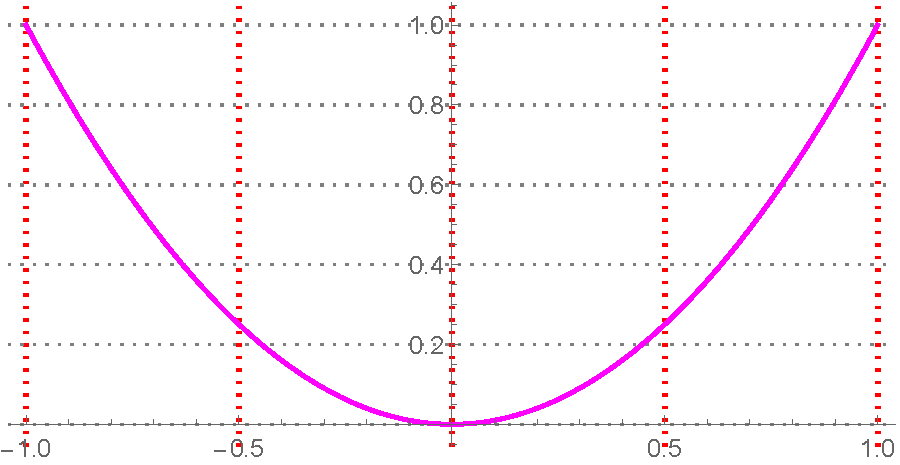
\includegraphics[scale=.85]{images/gridStyle}
\end{figure}

	\begin{itemize}
		\item[] Aumentando-se a proporção do gráfico vê-se que a primeira lista de valores contendo \ttt{Red}, \ttt{Dotted} e \ttt{Thick} gerou linhas verticais vermelhas, pontilhadas e, como foi passado o \ttt{Thick}, houve uma leve aumentada na espessura somente para melhorar a visualização do leitor.
	\end{itemize}

	\end{itemize}

	\newpage
	\vspace{.5cm}
	Para o \ttt{Plot3D} (Gráficos em 3d no geral) 
	\begin{itemize}
		\item\ttt{BoxRatios}
		\begin{itemize}
			\item Esse atributo é análogo ao \ttt{AspectRatio}, porém fazemos sua aplicação para três dimensões com base numa lista de três posições indicando a proporção em cada eixo como segue
			
\begin{lstlisting}[language=Mathematica]
Plot3D[x^2+y^2,{x,-1,1},{y,-1,1},BoxRatios->{1,1,1}]
\end{lstlisting}
			\begin{figure}[!h]
				\centering
				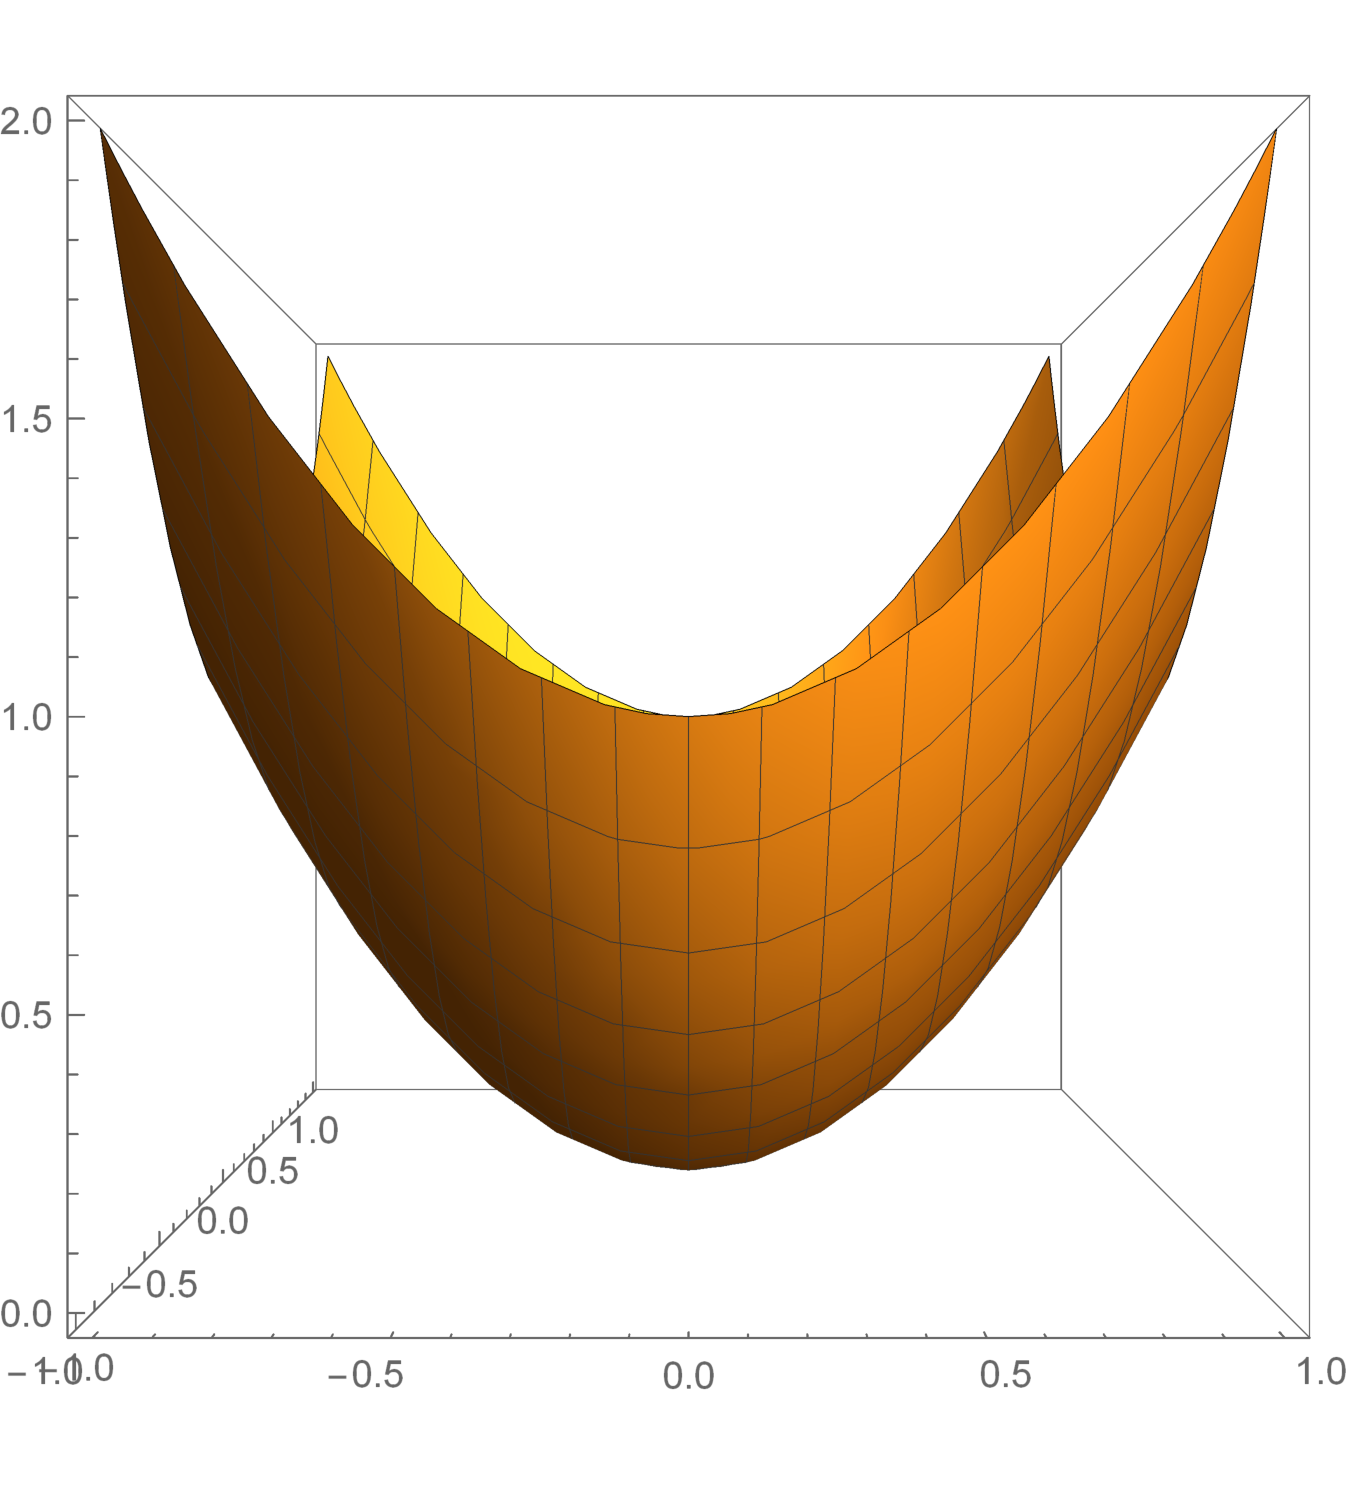
\includegraphics[scale=.35]{images/boxRatios}
			\end{figure}
			Como é visto, a proporção do gráfico foi aumentada ocasionando um estreitamento de sua base e aumento de sua altura na escala. 
			
			Caso quiséssemos testar fazendo uma figura com o eixo $z$ com metade da proporção, note a diferença

\begin{lstlisting}[language=Mathematica]
Plot3D[x^2+y^2,{x,-1,1},{y,-1,1},BoxRatios->{1,1,.5}]
\end{lstlisting}

		\begin{figure}[!h]
			\centering
			\includegraphics[scale=.35]{images/metadeboxRatios}
		\end{figure}

		\end{itemize}
		\item\ttt{Filling}
		\begin{itemize}
			\item Ferramenta bastante útil na estilização dos gráficos, nos permite criar um sombreado preenchendo a parte inferior das superfícies. Também é aplicável no \ttt{Plot}
			
\begin{lstlisting}[language=Mathematica]
Plot3D[x^2+y^2,{x,-1,1},{y,-1,1},Filling->Bottom]
\end{lstlisting}
			
			\begin{figure}[!h]
				\centering
				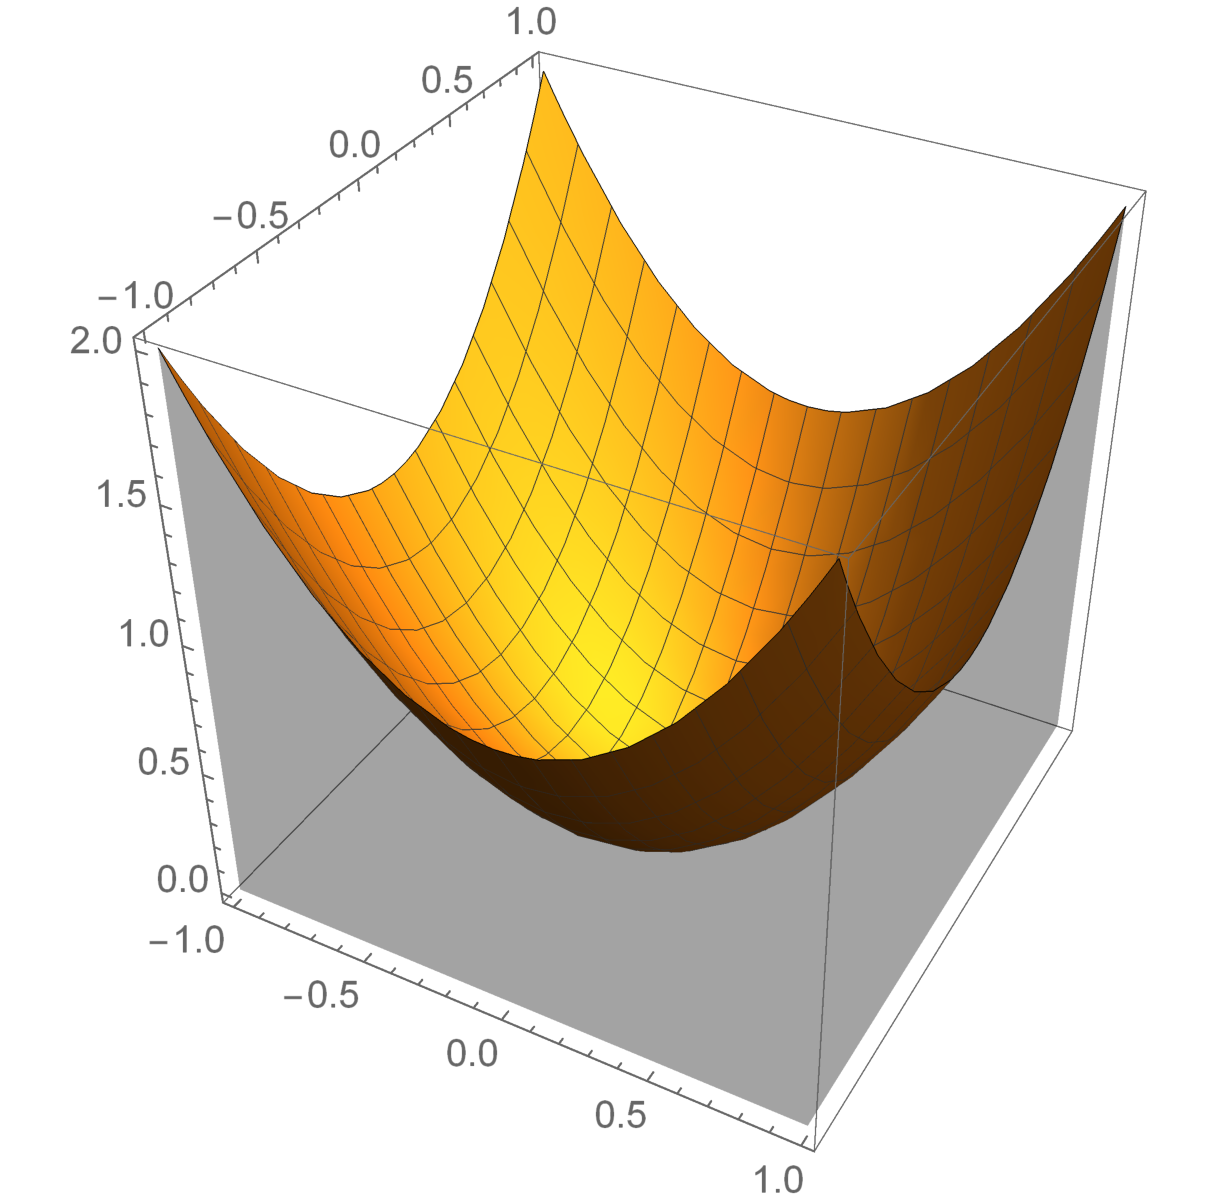
\includegraphics[scale=.45]{images/Filling}
			\end{figure}
			
			\begin{itemize}
				\item Aplicando o \ttt{FillingStyle}, até então não mencionado podemos obter
				
\begin{lstlisting}[language=Mathematica]
Plot3D[x^2+y^2,{x,-1,1},{y,-1,1},Filling->Bottom,FillingStyle->Opacity[.8],PlotStyle->Red]
\end{lstlisting}

				\begin{figure}[!h]
					\centering
					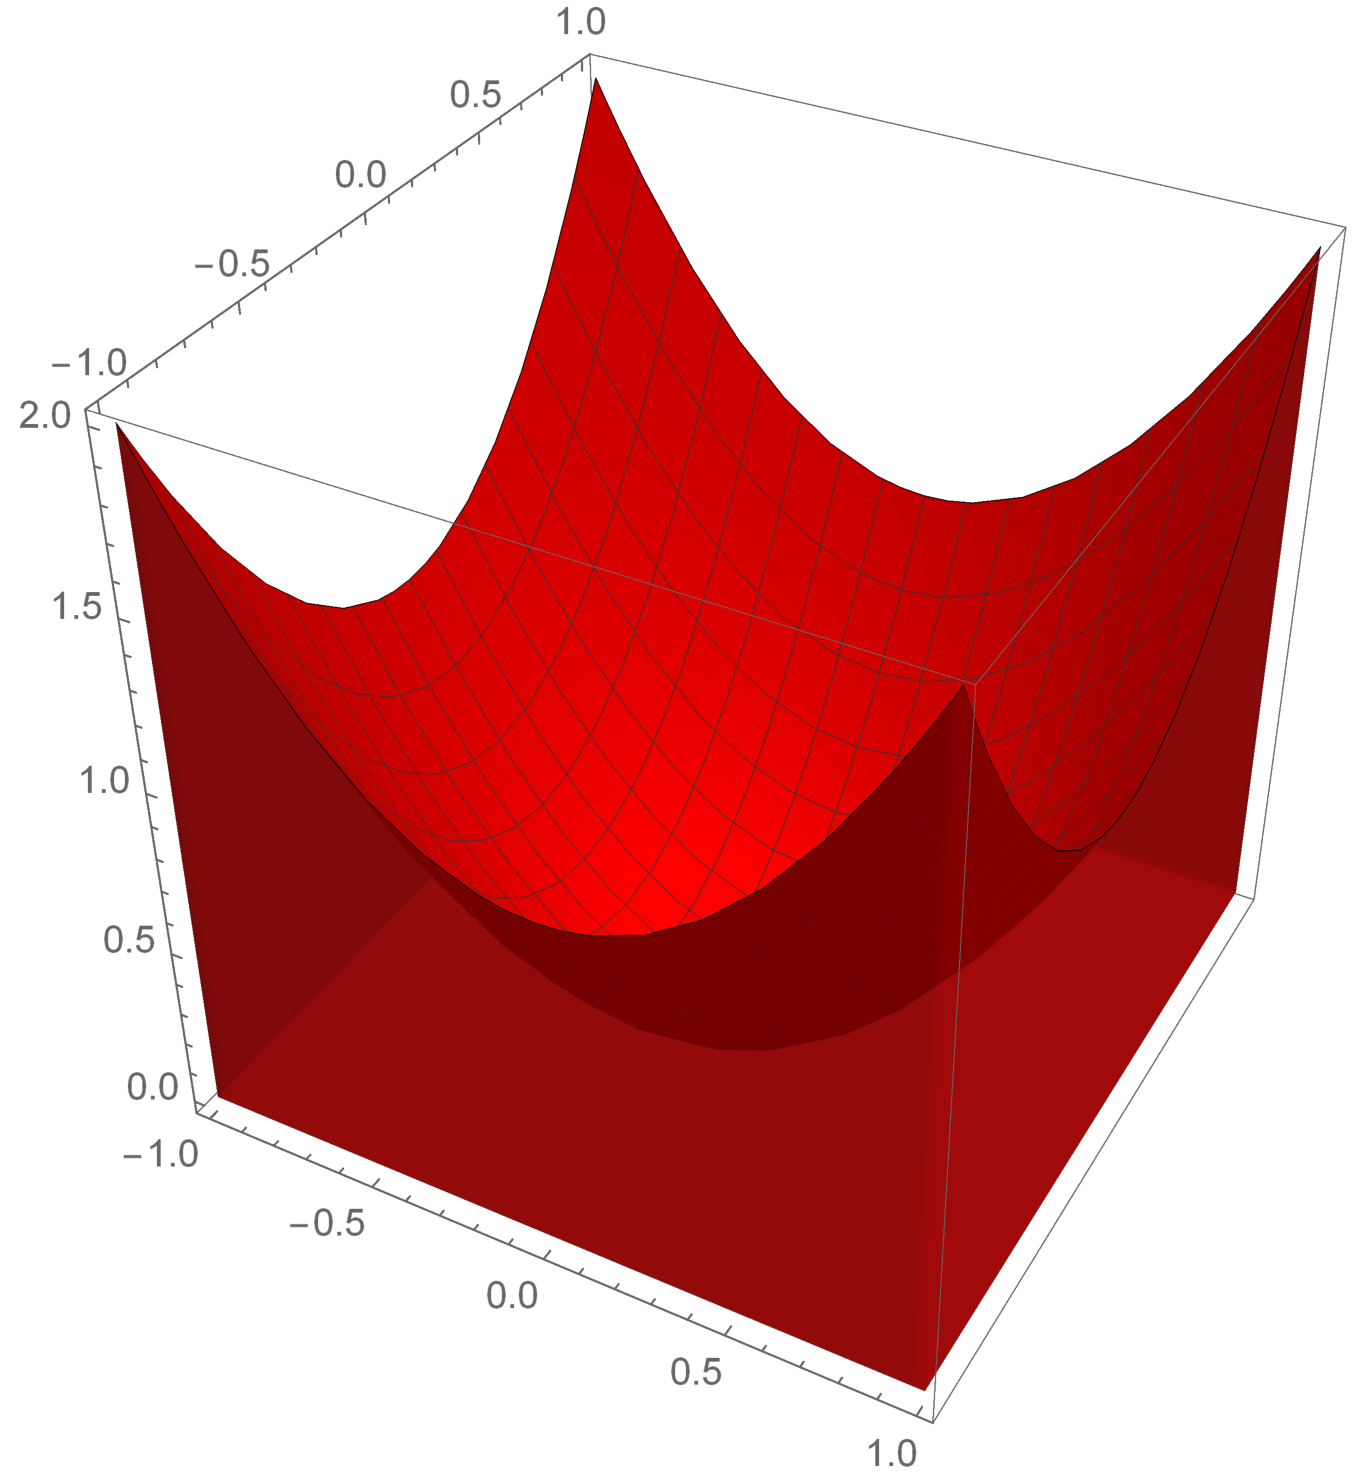
\includegraphics[scale=.35]{images/FillingStyle}
				\end{figure}
			\end{itemize}
		
		\end{itemize}
		\item\ttt{BoundaryStyle}
		
			Cria um contorno ao longo das bordas da superfície.
\begin{lstlisting}[language=Mathematica]
Plot3D[x^2+y^2,{x,-1,1},{y,-1,1},BoundaryStyle->{Thick,RGBColor[0,255,255]}]
\end{lstlisting}
			
			\begin{figure}[!h]
				\centering
				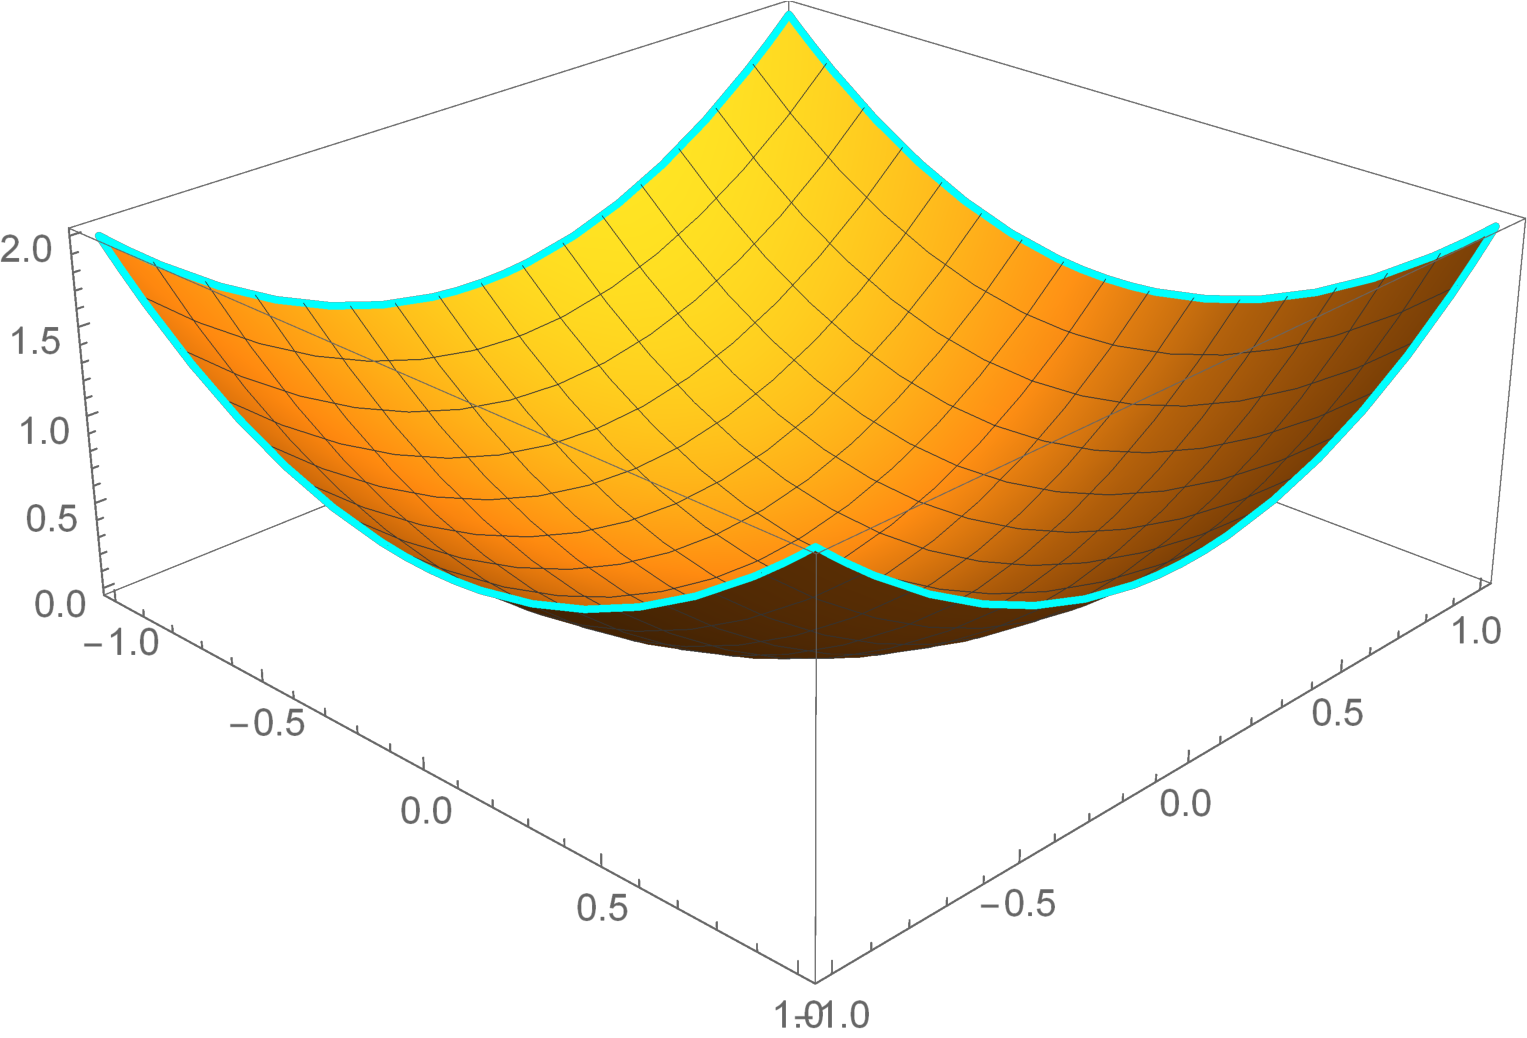
\includegraphics[scale=.25]{images/BoundaryStyle}
			\end{figure}
		
		\item\ttt{PlotStyle}
			
			Vamos resgatar algumas propriedades de estilização já conhecidas mostrando alguns exemplos de superfícies 

\begin{lstlisting}[language=Mathematica]
Plot3D[x^3+y^3,{x,-1,1},{y,-1,1},PlotStyle->{Green}, 
BoundaryStyle->{Thick,Blue},Filling->Bottom, 
FillingStyle->{Opacity[.2]},BoxRatios->{1,1,3}]
\end{lstlisting}

			\begin{figure}[!h]
				\centering
				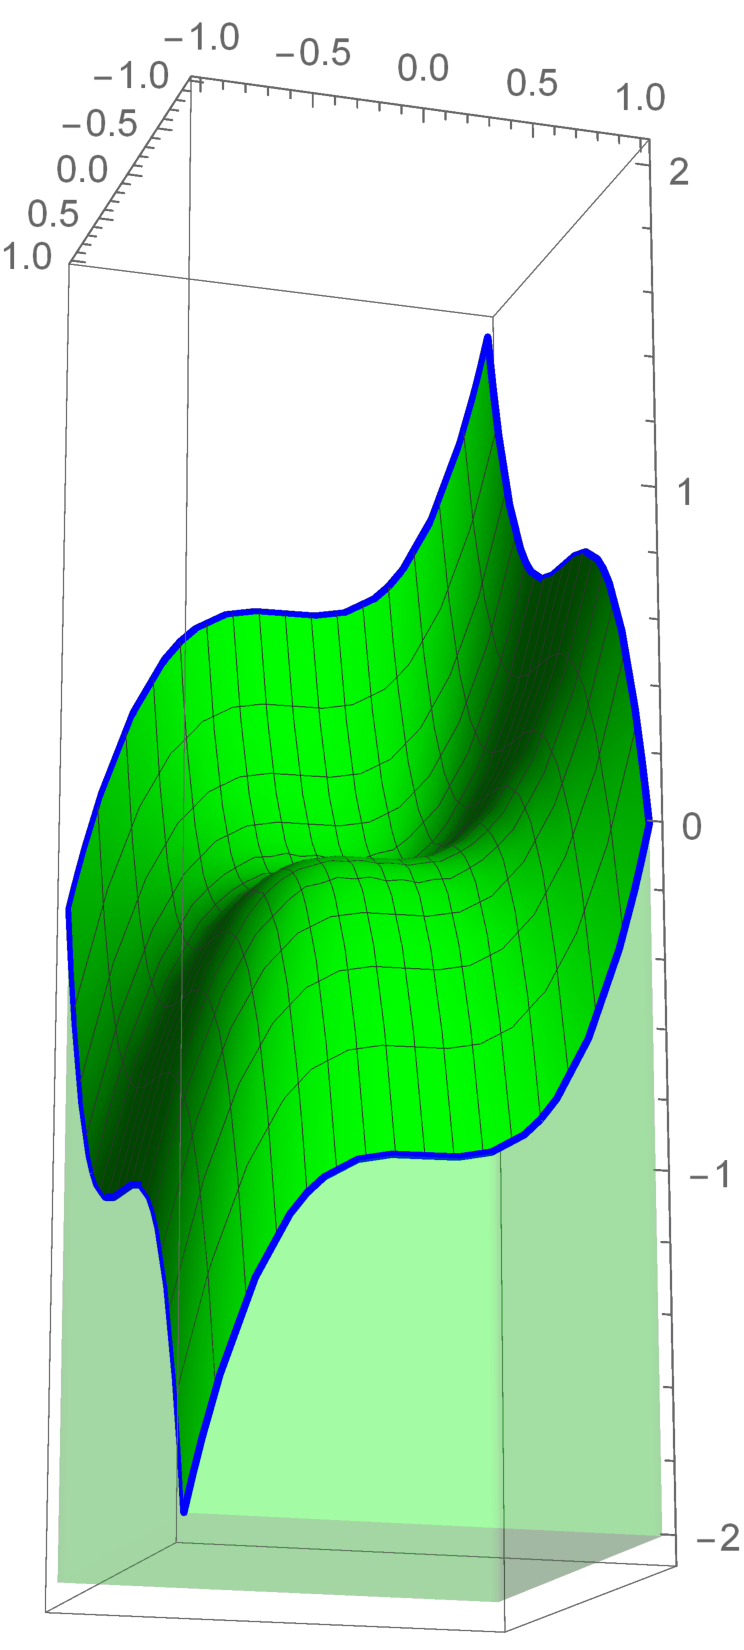
\includegraphics[scale=.2]{images/PlotStyle3d2}
			\end{figure}

\begin{lstlisting}[language=Mathematica]
Plot3D[x^2+y^2,{x,-1,1},{y,-1,1},PlotStyle-> {LightBlue},BoundaryStyle->{Thick,Blue},Filling-> Bottom,FillingStyle->{Opacity[.2]}]
\end{lstlisting}

			\begin{figure}[!h]
				\centering
				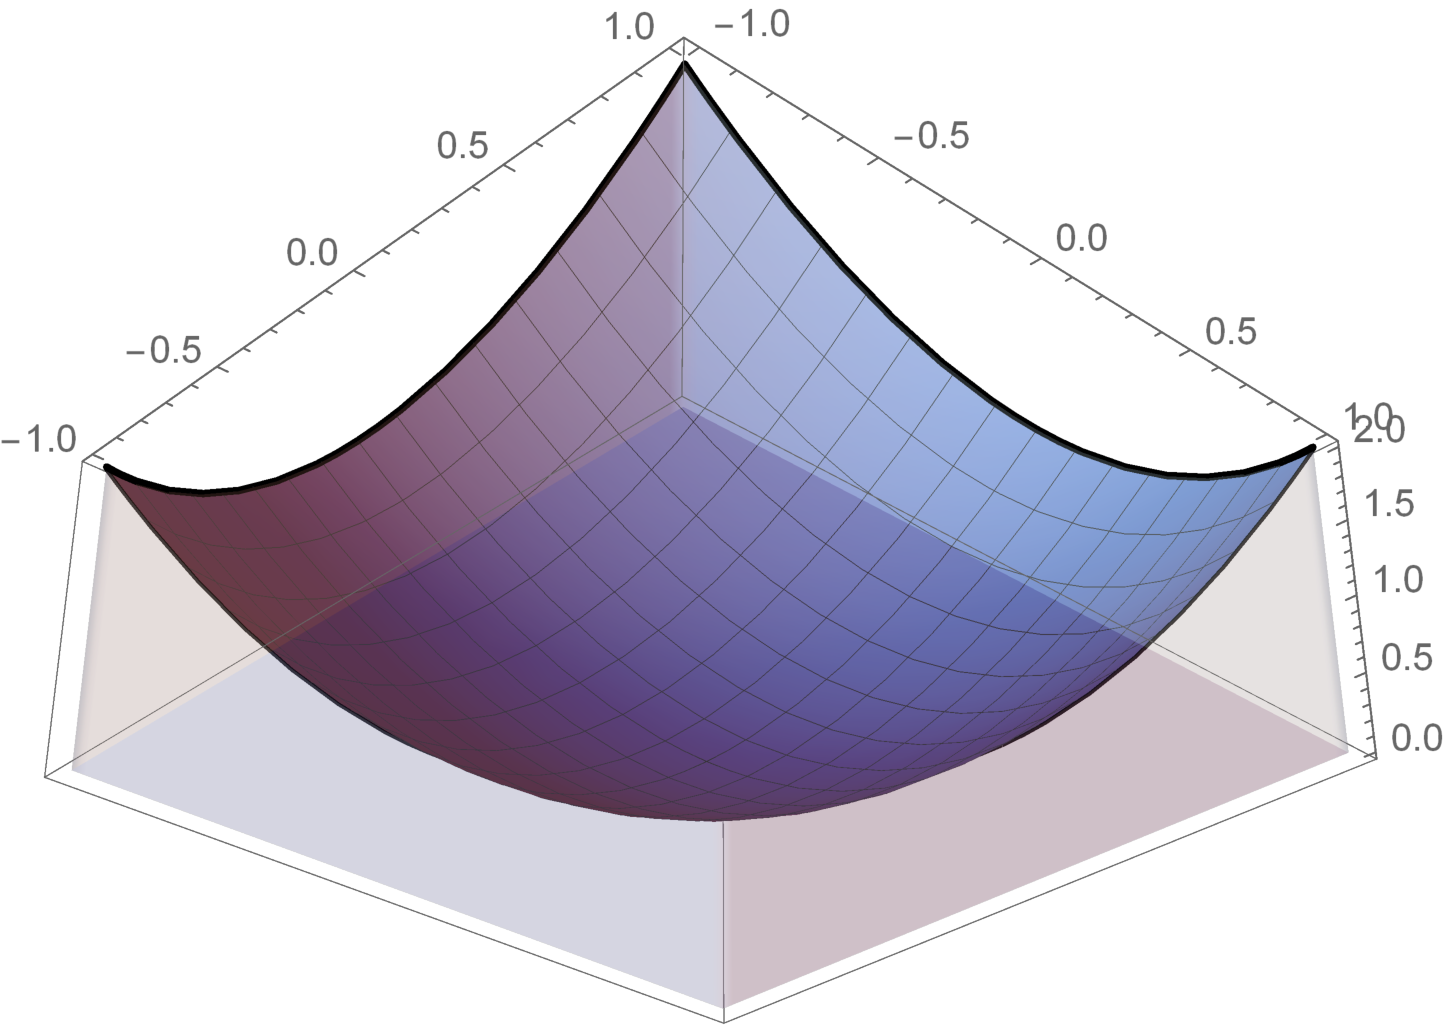
\includegraphics[scale=.3]{images/PlotStyle3d1}
			\end{figure}
	\end{itemize}

	\section{ContourPlot}
		Esse comando nos permite plotar os contornos de funções a depender de como passamos os parâmetros. Podemos imaginar que caso passarmos uma expressão seguindo a mesma estrutura do \ttt{Plot} vamos ter a replicação da função $f$ ao longo do eixo $y$ em diferentes alturas. Vamos exemplificar para tornar mais fácil.
		
		Imagine que desejamos novamente plotar a função do segundo grau $f(x)=x^{2}$, só que dessa vez, ao invés de plotar somente uma curva queremos uma família de funções que seguem o mesmo molde porém transladadas em $y$. Dessa forma, passaríamos o comando como é visto abaixo 
		
\begin{lstlisting}[language=Mathematica]
ContourPlot[y-x^2,{x,-1,1},{y,-1,1}]
\end{lstlisting}

\begin{figure}[!h]
	\centering
	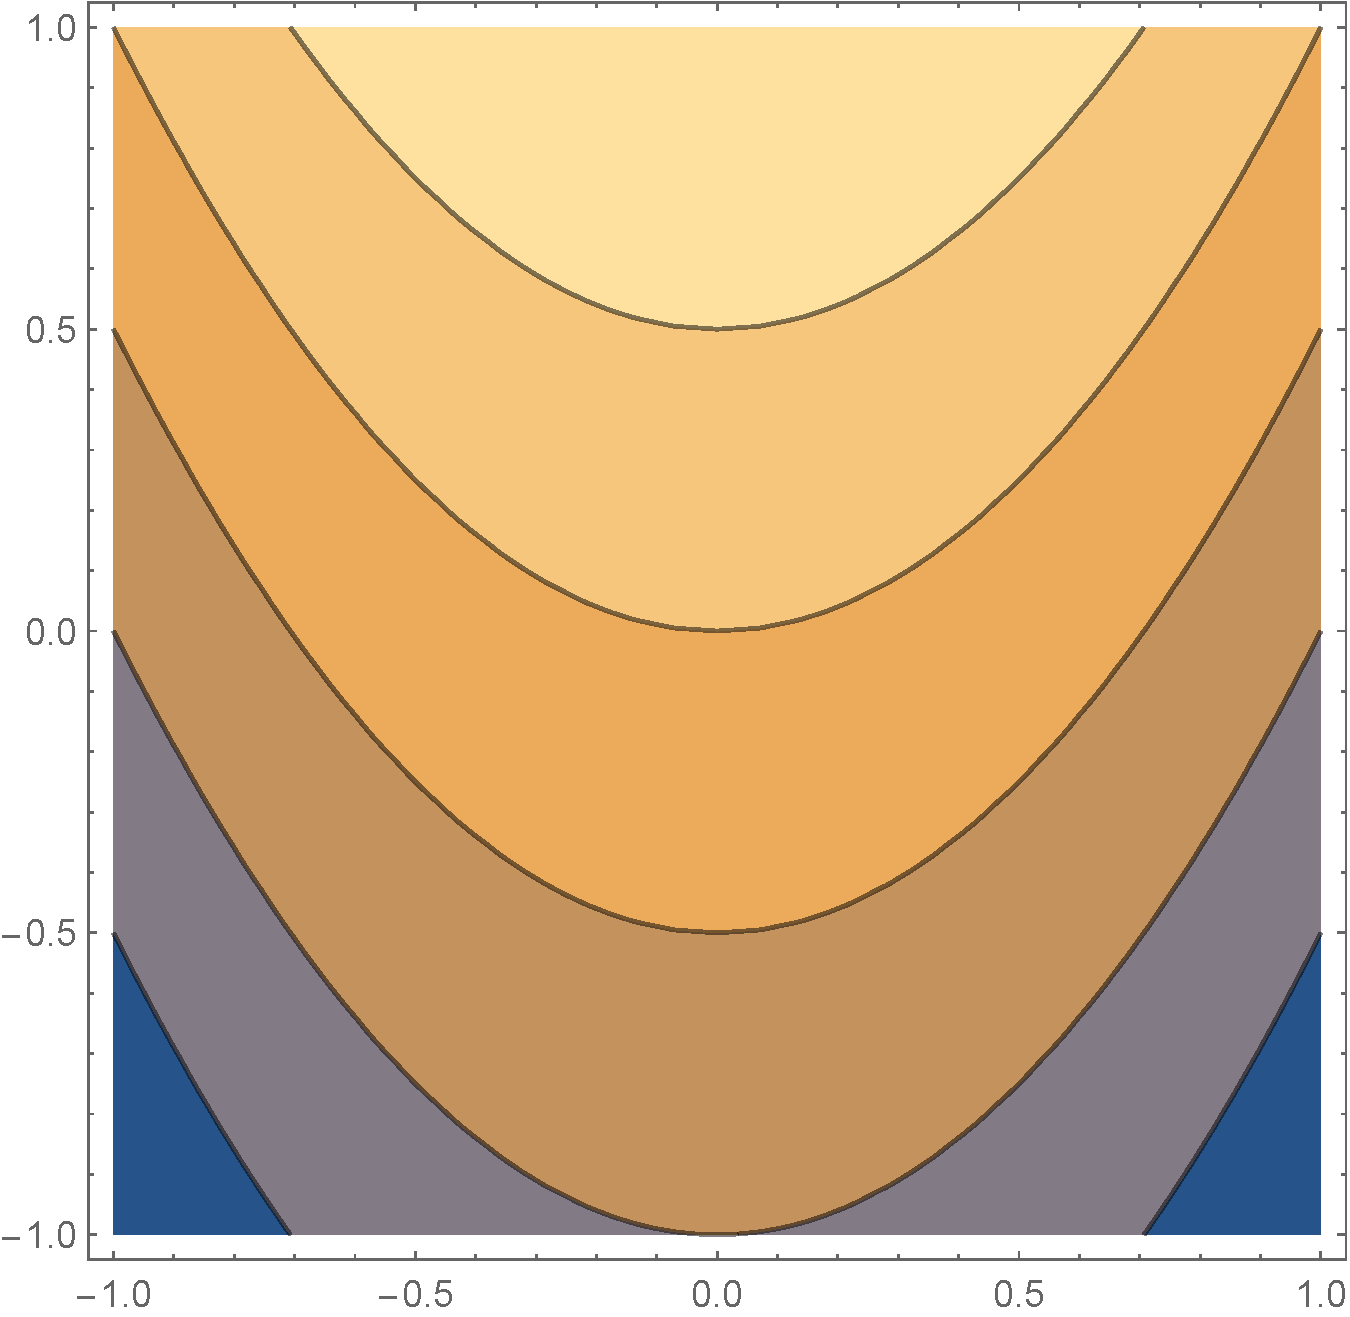
\includegraphics[scale=.27]{images/ContourPlot}
\end{figure}

	Afinal, o que foi feito para que chegássemos nessa conformação de curvas? A resposta é simples: Simplesmente assumimos que $f(x)=x^{2}$, trocamos $f(x)$ por $y$ e subtraímos $x^{2}$ de ambos os lados, logo
	
	\begin{equation}
		y-x^{2}=0
	\end{equation}
	
	Isso significa que temos um contorno da função $f$ cujo rótulo corresponde a 0. Ou seja, o valor nulo encontrado demonstra que a função $f$ ao longo de toda a curva $y-x^{2}$ está rotulado como 0 em três dimensões (Altura constante ao longo dessa parábola). É importante lembrar que ao igualar a 0, podemos imagina uma nova função $g$, dependente de $x$ e $y$ que descreve os contornos no espaço. Ou seja. no lugar de chamarmos os contornos por $k$, para designar uma constante associada ao $label$ da curva de nível, usamos $g$ e a reescrevemos como
	
	\begin{equation}
		g(x,y)=y-x^{2}
	\end{equation}
	
	
	
	Nesse caso, como estamos tratando de rótulos um atributo interessante de ser usado é o \ttt{ContourLabels}. Ele vai mapear a altura de cada parábola na representação em duas dimensões. Vejamos

\begin{lstlisting}[language=Mathematica]
ContourPlot[y-x^2,{x,-1,1},{y,-1,1},ContourLabels-> True,ContourShading->False]
\end{lstlisting}

	\newpage
	\begin{figure}[!h]
		\centering
		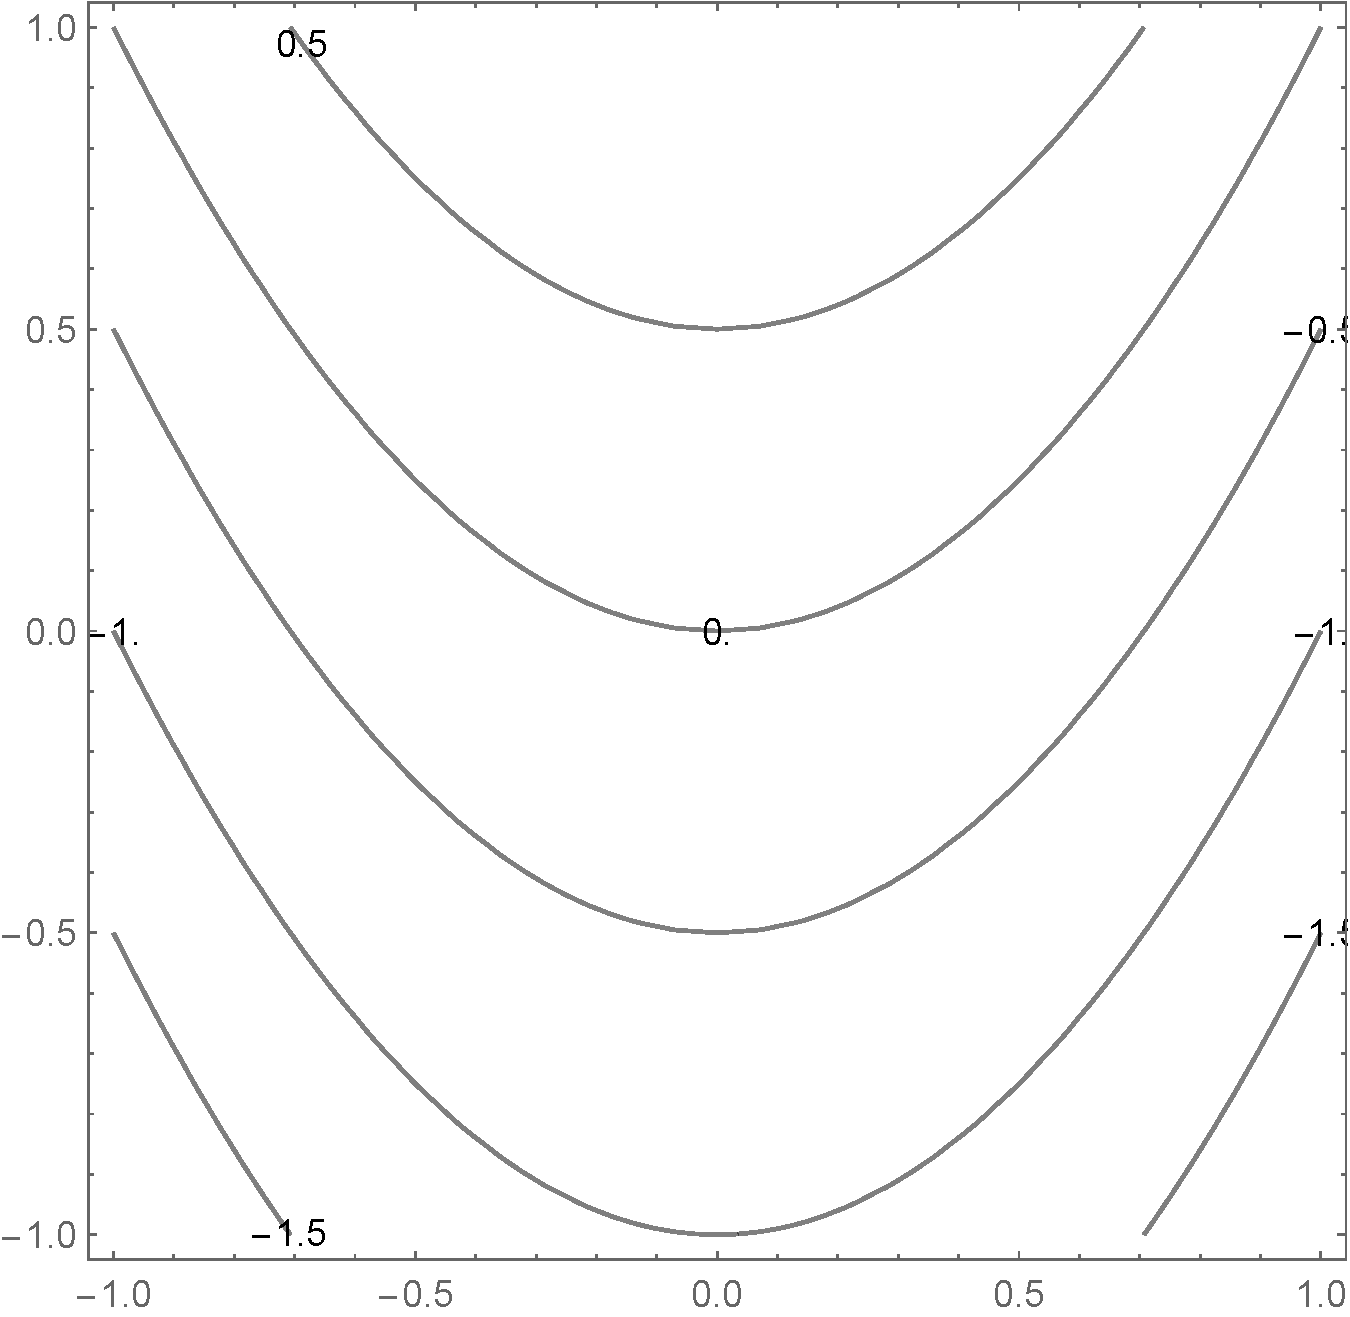
\includegraphics[scale=.47]{images/ContourLabels}
	\end{figure}

	Vemos o mapa de contornos referido. Para melhorar a visualização empregou-se o \ttt{ContourShading->False}. Note que o \textit{label} 0. indica o contorno que foi discutida anteriormente. Para comprovarmos, usando o \ttt{ContourPlot}, vamos reforçar essa parábola com base na equação do contorno $y-x^{2}=k$, onde $k$ corresponde ao contorno 0.
	
\begin{lstlisting}[language=Mathematica]
Show[ContourPlot[{y-x^2},{x,-1,1},{y,-1,1},ContourLabels->True,ContourShading->False,GridLines->Automatic],ContourPlot[
y-x^2==0,{x,-1,1},{y,-1,1},ContourStyle->{Thick,Blue}]]
\end{lstlisting}

	\begin{figure}[!h]
		\centering
		\includegraphics[scale=.37]{images/ContourZero}
	\end{figure}

	Repare que utilizou-se o \ttt{Show} para juntarmos os dois \ttt{ContourPlot}s. O primeiro representa os vários contornos \ttt{y-x\^\,\!2\,==\,k}, enquanto o segundo o contorno de rótulo nulo.
	
	Usando esse tópico de âncora vamos falar do \ttt{ContourPlot3D}. Imagina se quiséssemos representar esse contorno com $k=0$ no espaço. Com base no gráfico em 2d ao olhar de cima para baixo notamos que a parábola superior possui $k=0.5$ e vai diminuindo até $k=-1.5$. Isso demonstra que a superfície está diminuindo sua altura nesse intervalo com base na interpretação desses vários valores de $k$ (ou curvas de nível). Vejamos como fica em três dimensões
	
\begin{lstlisting}[language=Mathematica]
superficie = ContourPlot3D[z==y-x^2,{x,-1,1},{y,-1,1},{z,-1.6,.6}, 
ContourStyle->{Blue,Opacity[0.3]},BoundaryStyle->{Thick,Blue}]
\end{lstlisting}

	\begin{figure}[!h]
		\centering
		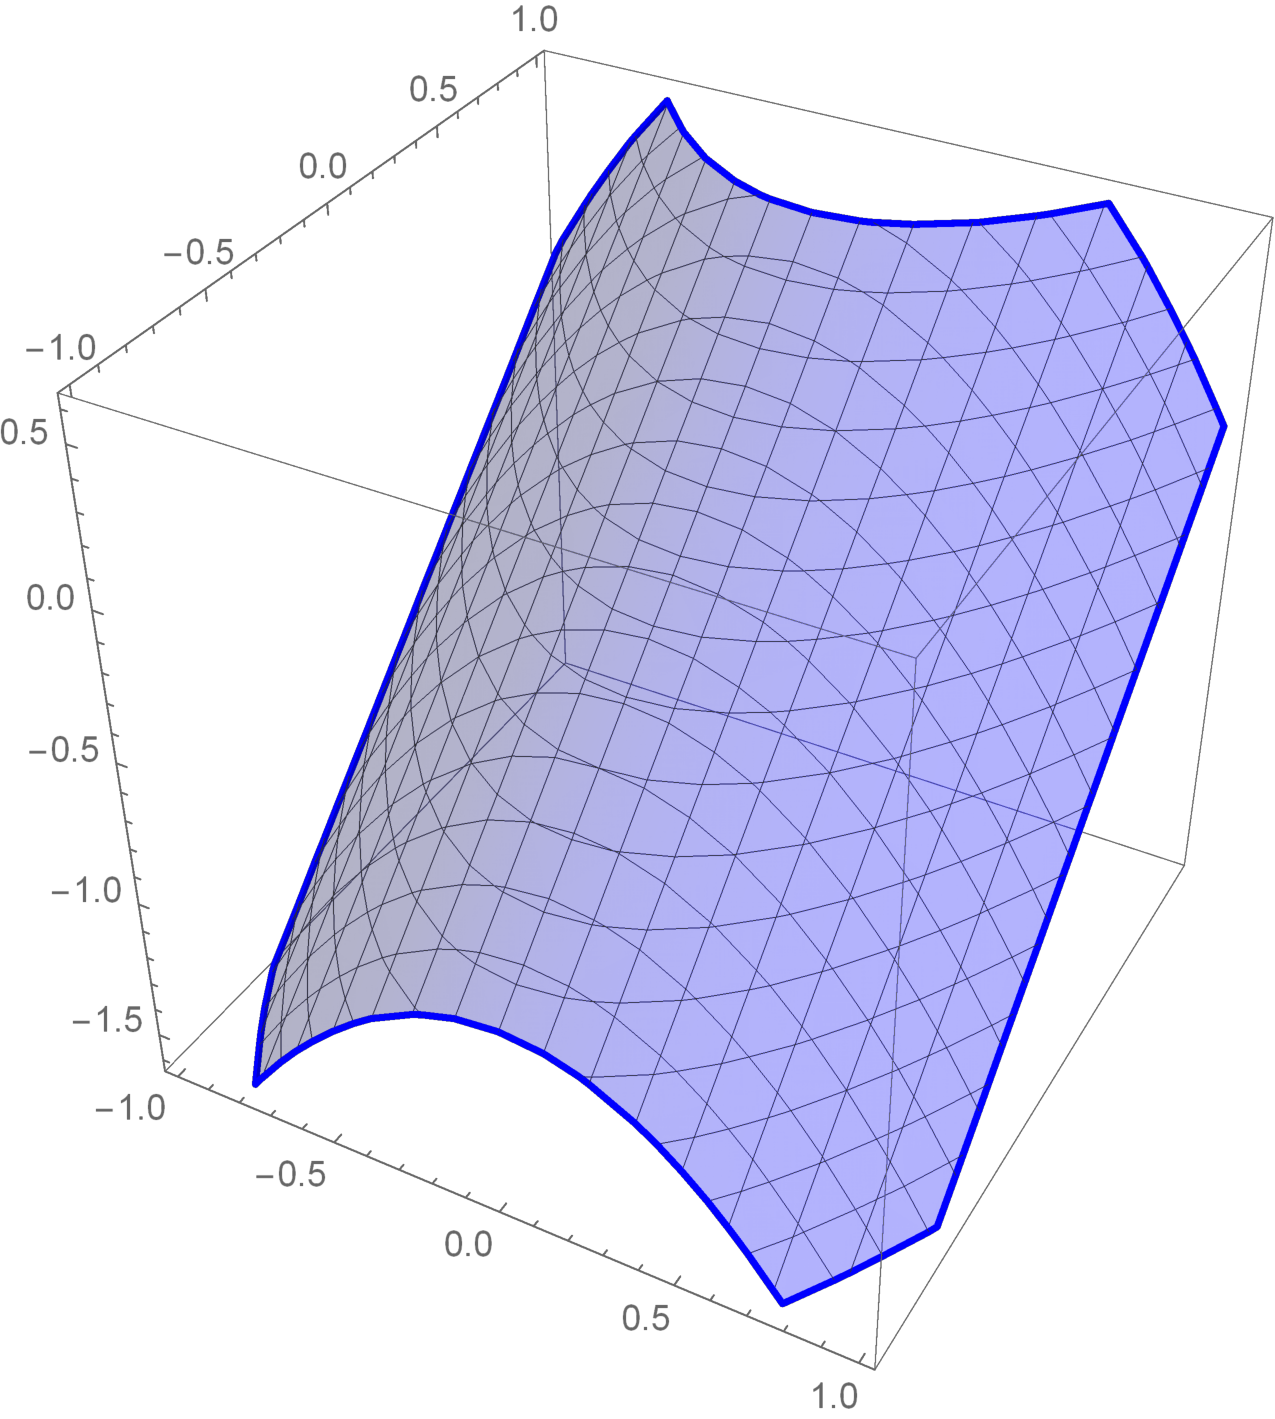
\includegraphics[scale=.3]{images/ContourPlot3d}
	\end{figure}

	O gráfico acima revela somente os vários valores de $k$ que agora podem ser interpretados de forma qualitativa. Se mudarmos a vista, podemos fazer a comparação das projeções\\
	
	\begin{minipage}{.5\linewidth}
		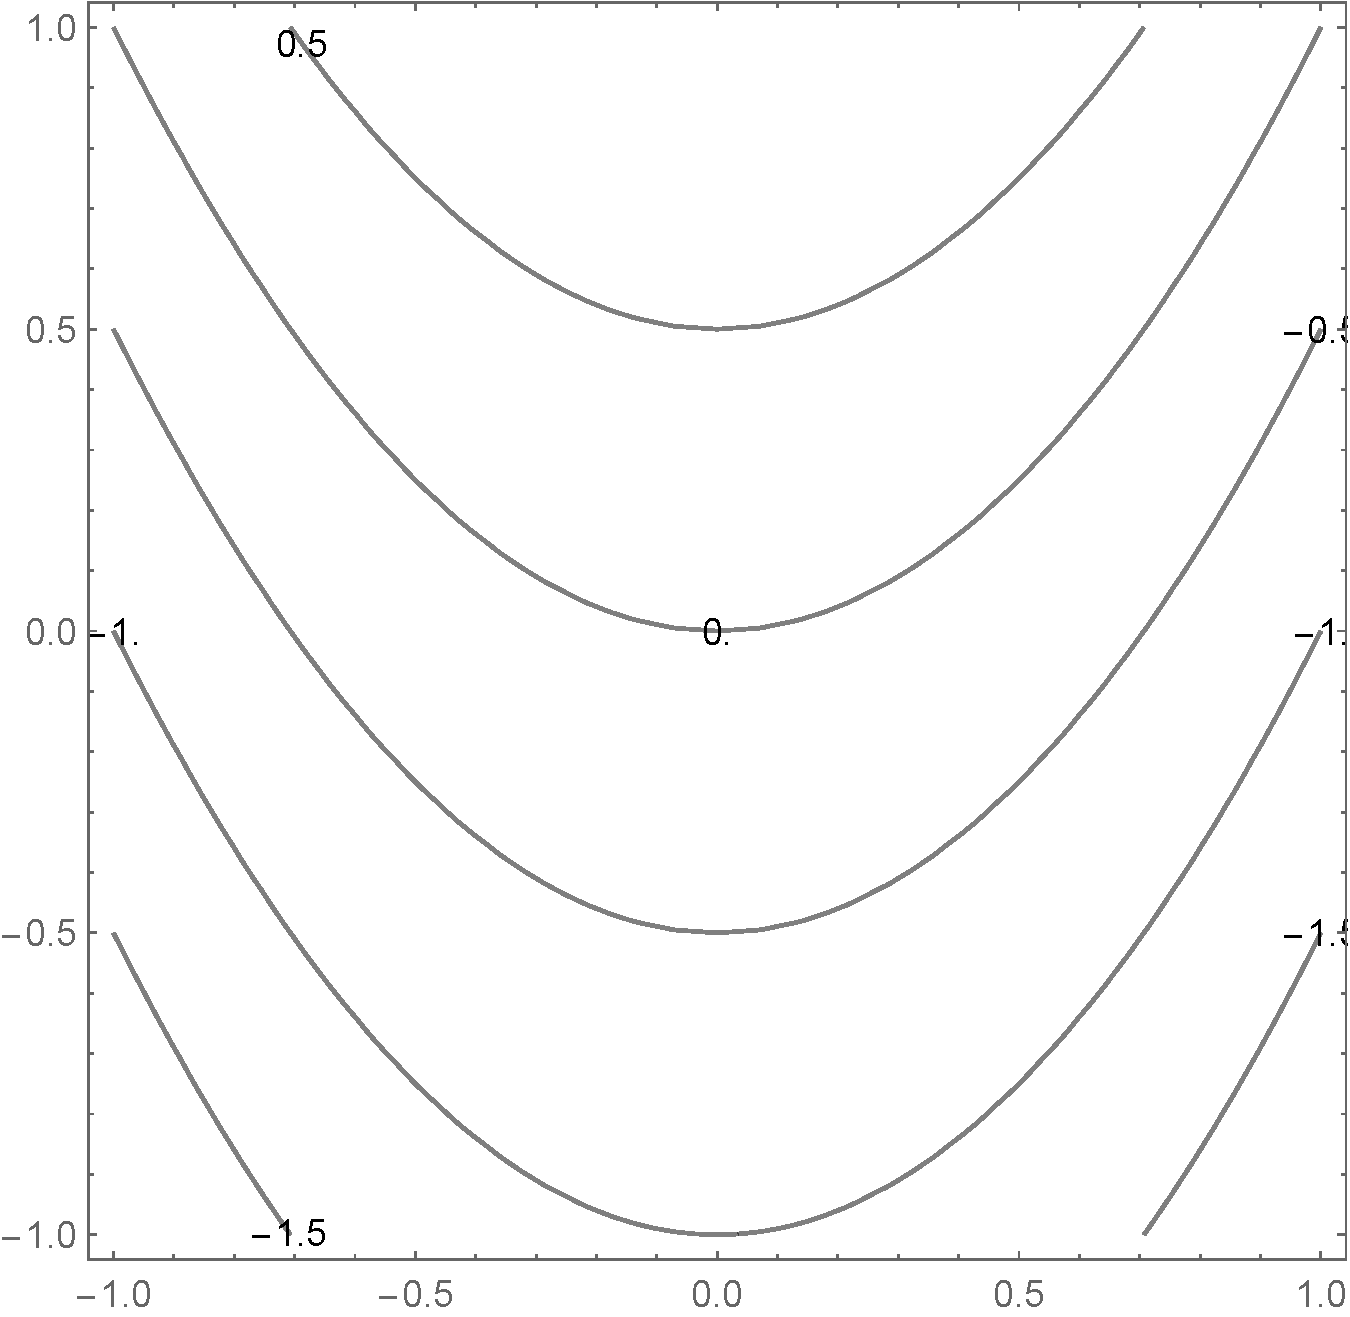
\includegraphics[scale=.24]{images/ContourLabels}
	\end{minipage}
	\begin{minipage}{.5\linewidth}
		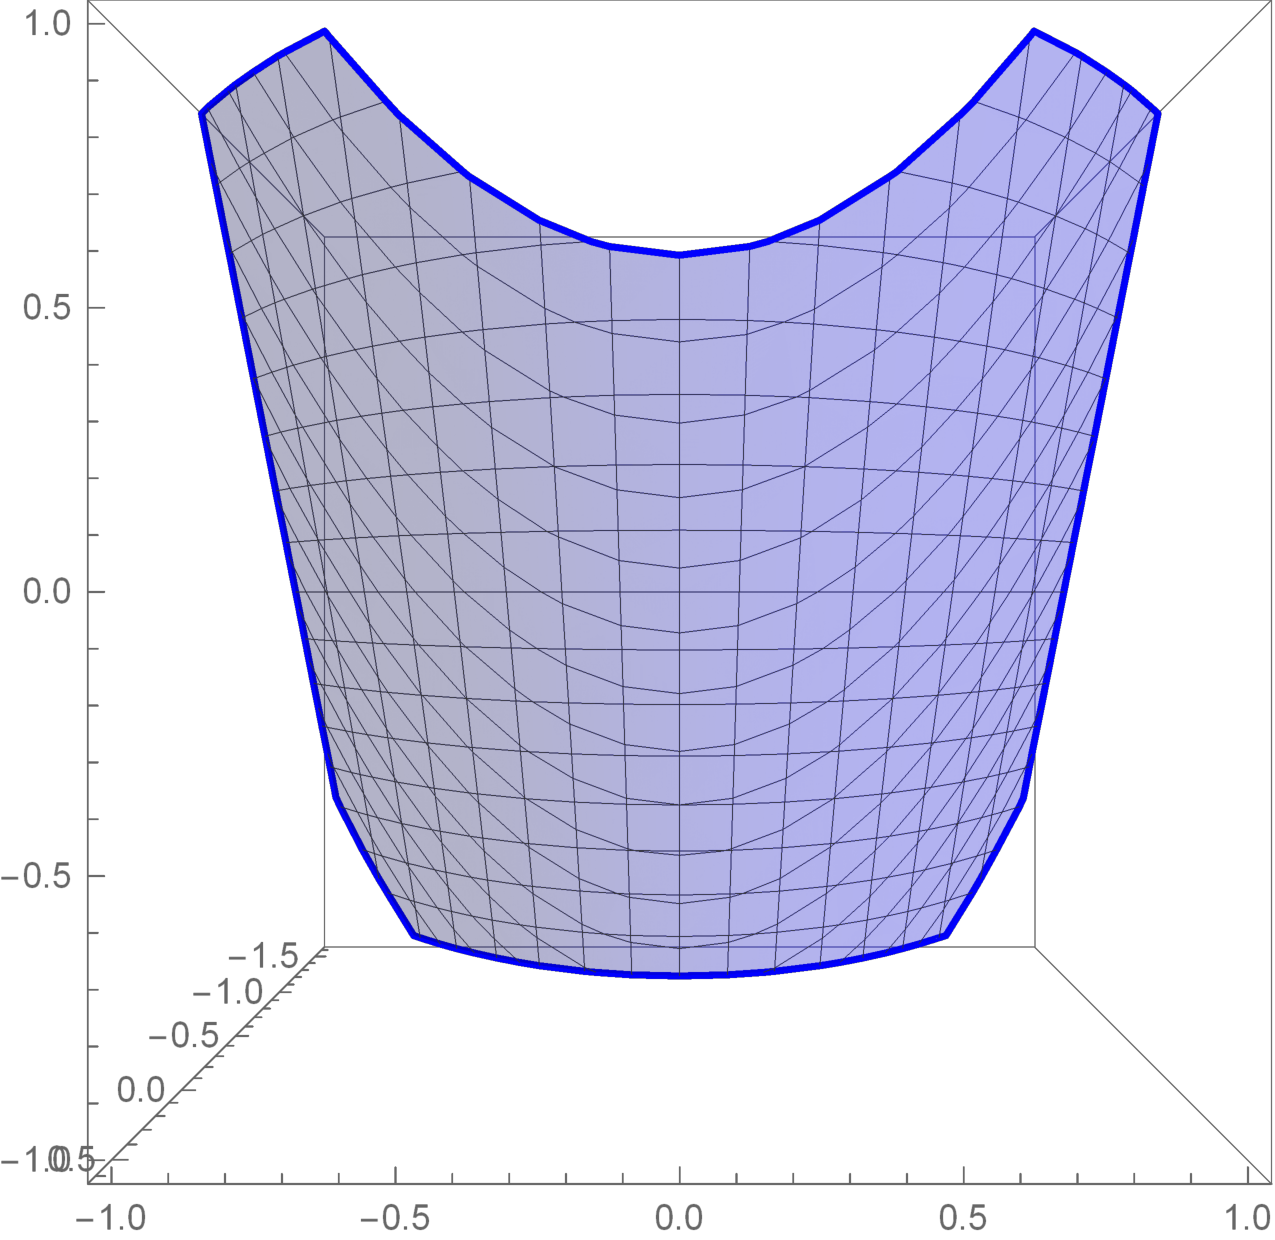
\includegraphics[scale=.25]{images/Top3dContours}
	\end{minipage}

	Um conceito importante está relacionado à ideia de que uma curva em duas dimensões, no espaço torna-se uma superfície. Tendo isso em mente, concluimos que a curva mais espessa identificada anteriormente para $k=0$ em duas dimensões, agora torna-se uma superfície que não depende de $z$. Vamos verificar
	
\begin{lstlisting}[language=Mathematica]
superficie2 = ContourPlot3D[0==y-x^2,{x,-1,1},{y,-1,1},{z,-1.6,.6},ContourStyle->{Red,Opacity[0.3]},BoundaryStyle->{Thick,Red}]
\end{lstlisting}

\begin{minipage}{.5\linewidth}
	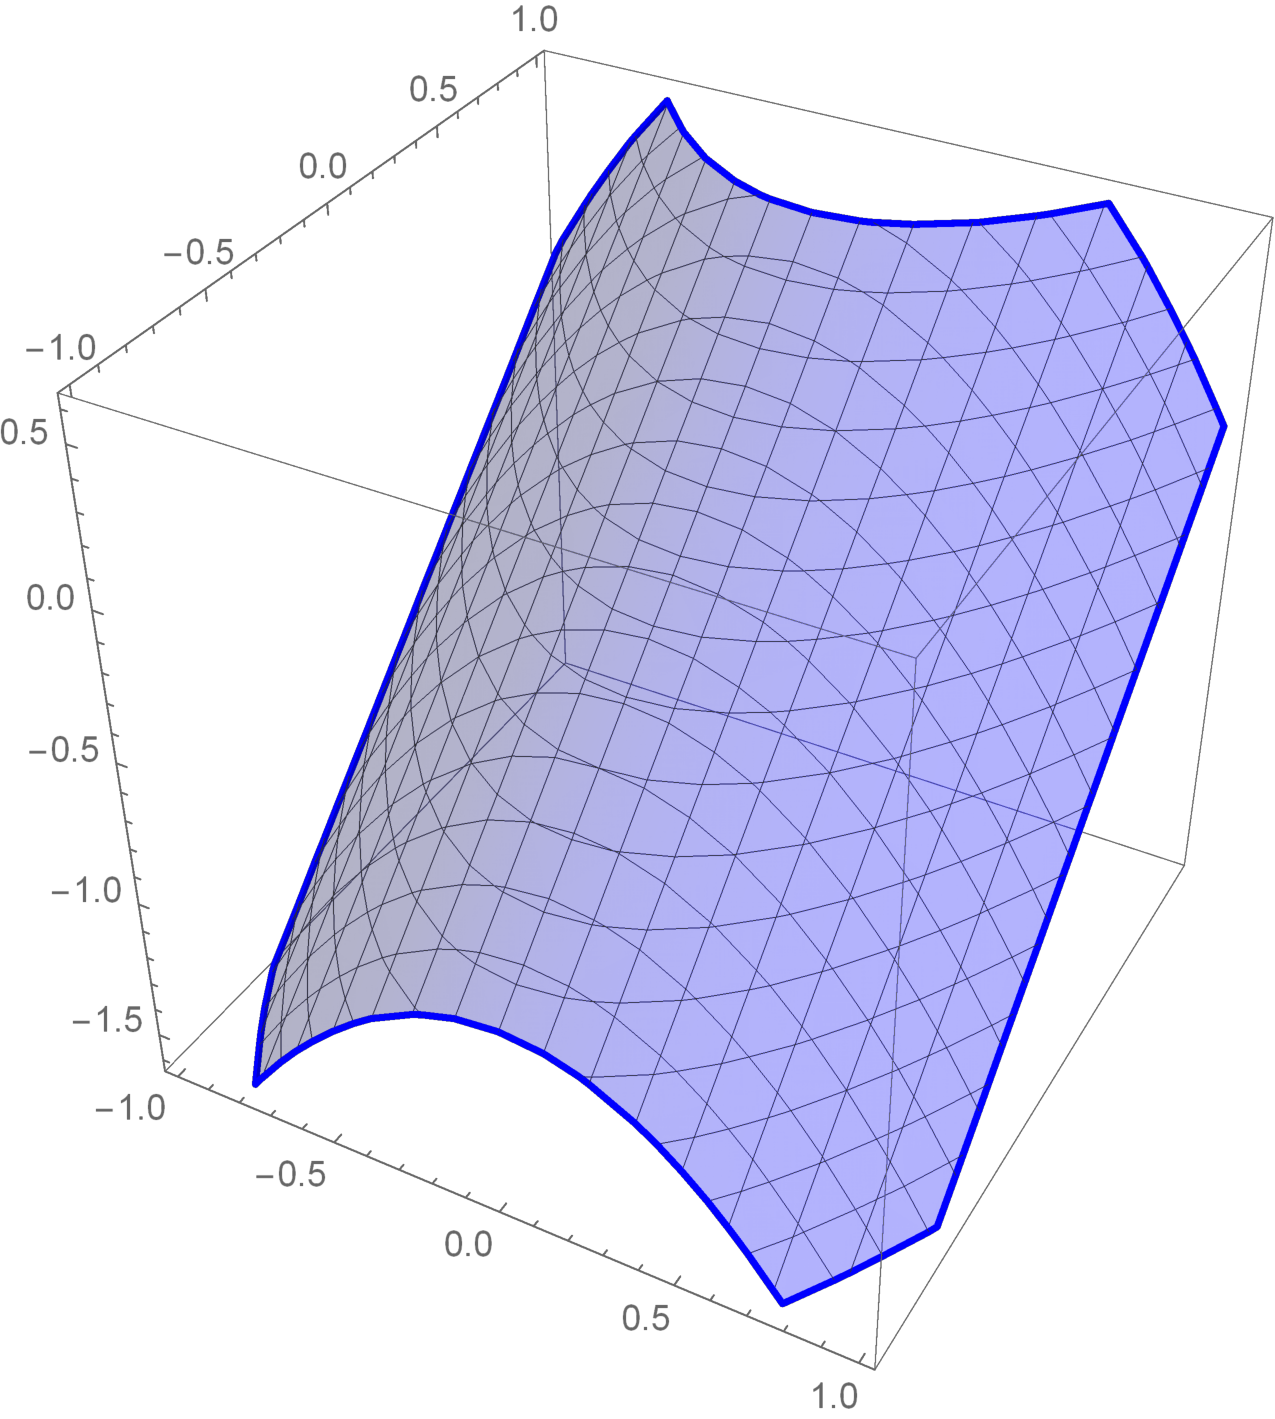
\includegraphics[scale=.25]{images/ContourPlot3d}
\end{minipage}
\begin{minipage}{.5\linewidth}
	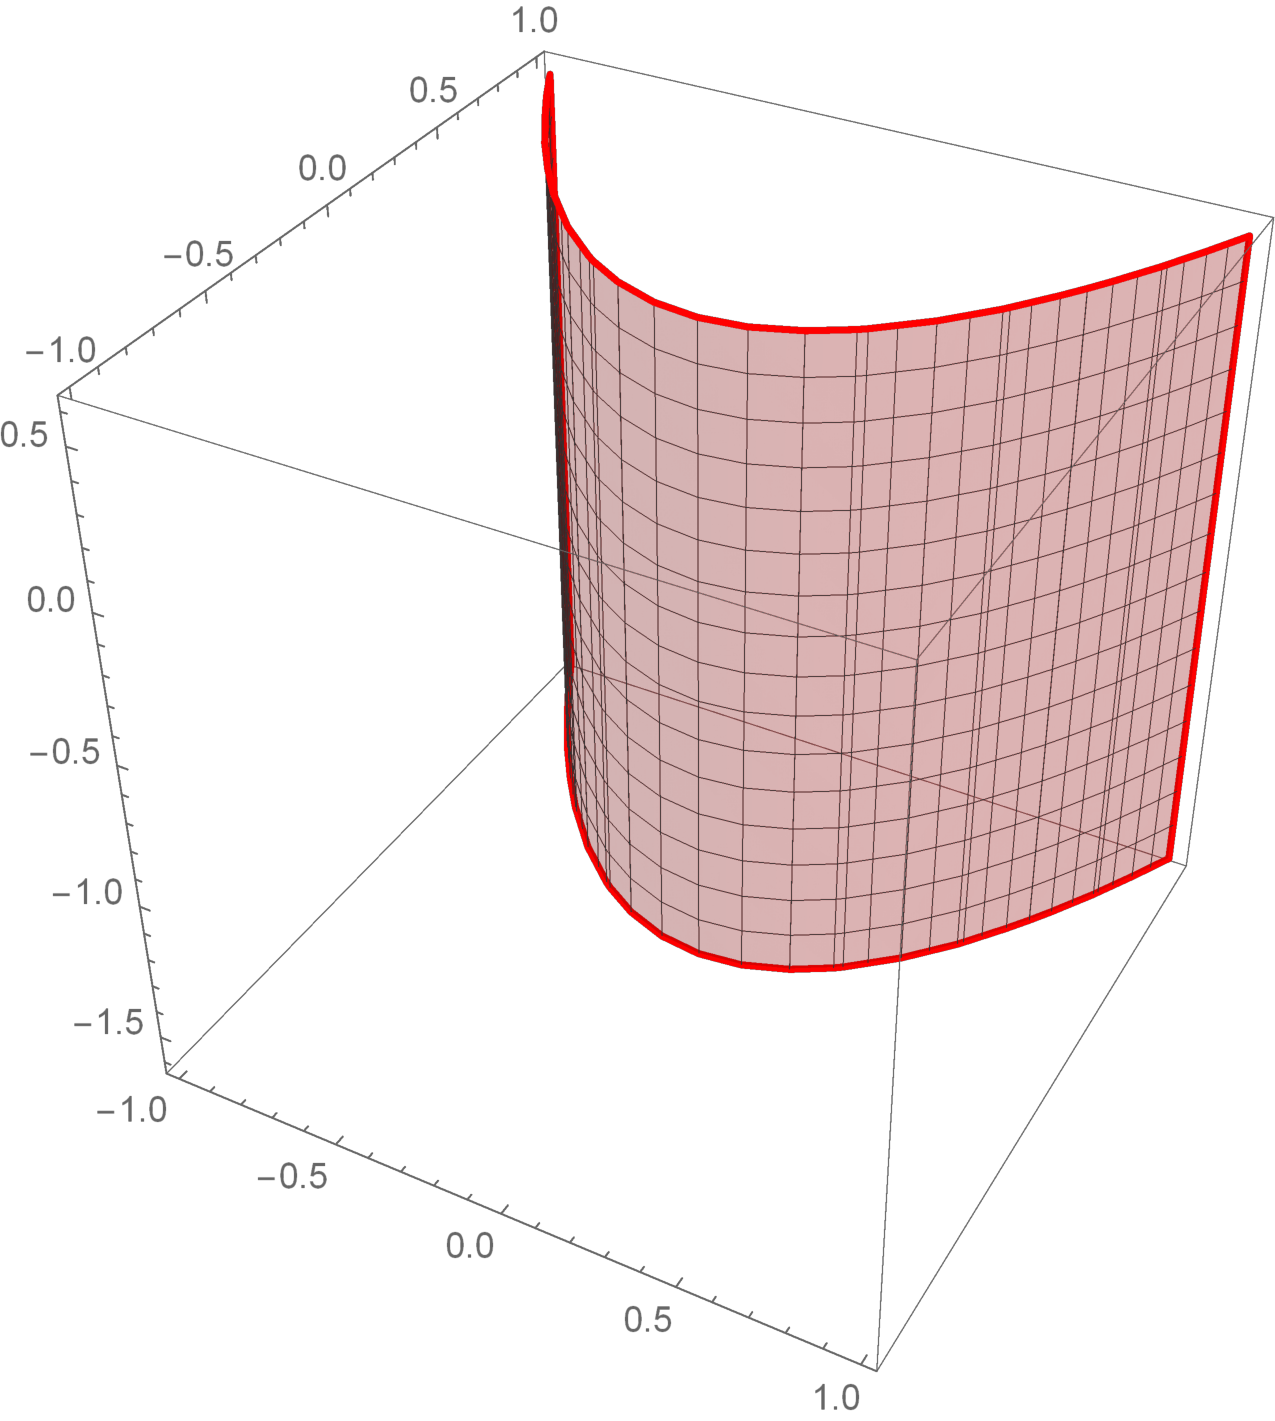
\includegraphics[scale=.25]{images/ContourRed}
\end{minipage}

Juntando as duas

\begin{lstlisting}[language=Mathematica]
Show[superficie,superficie2]
\end{lstlisting}

\begin{figure}[!h]
	\centering
	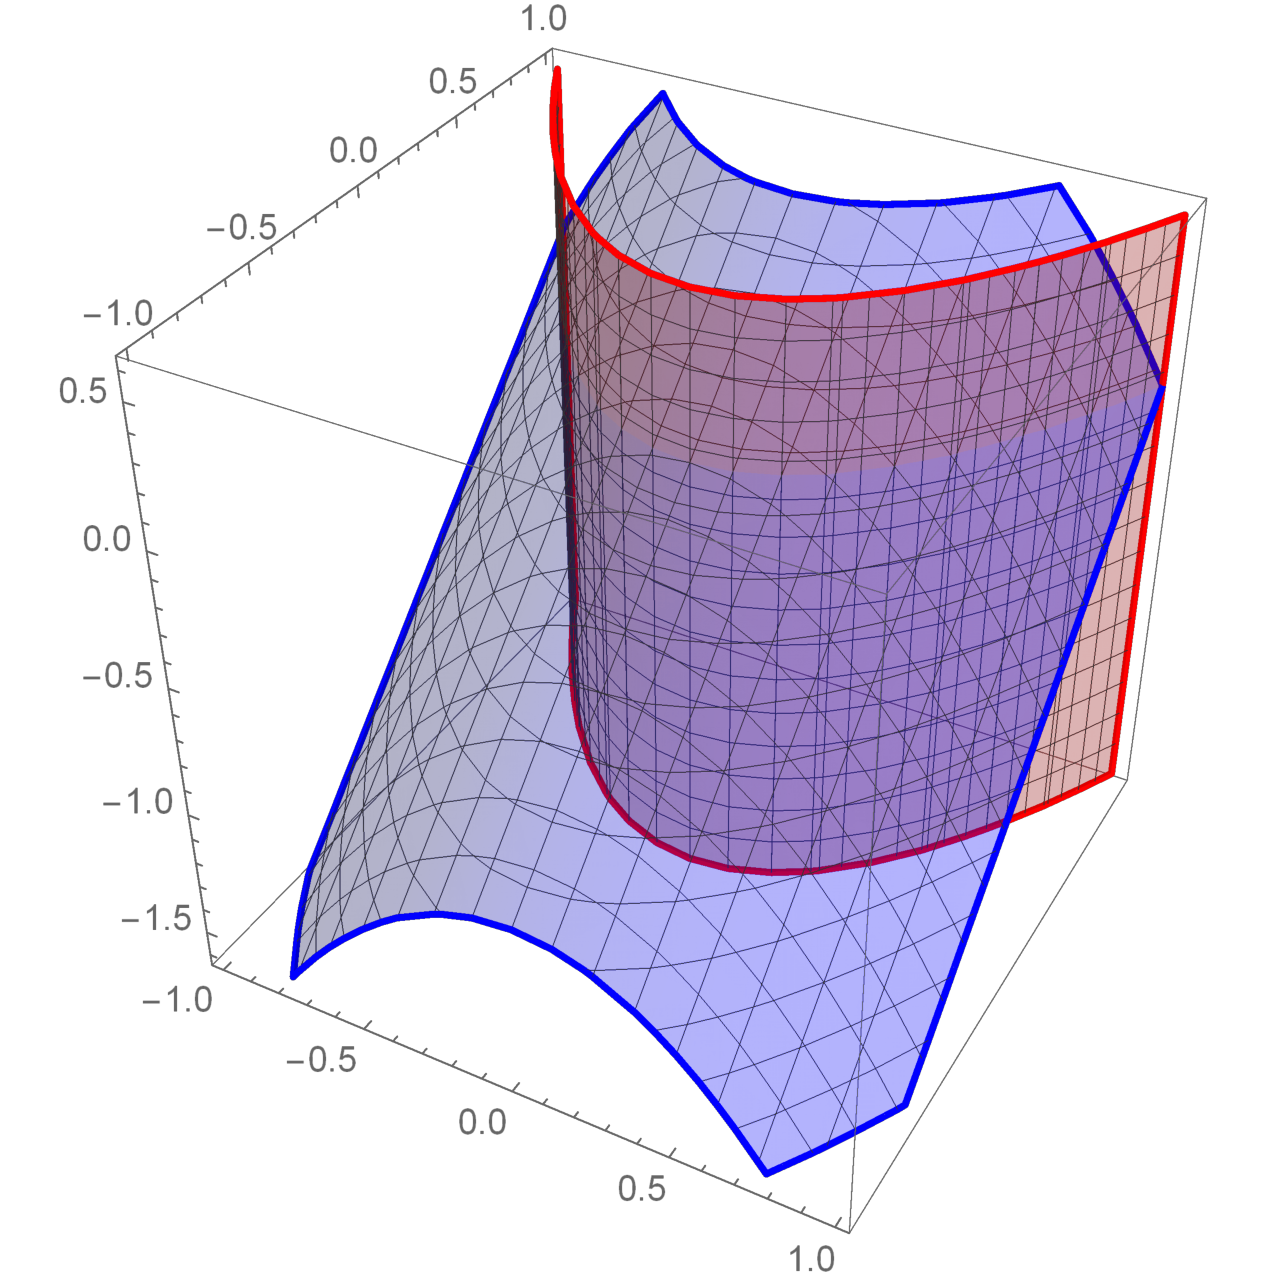
\includegraphics[scale=.44]{images/Juntos}
\end{figure}

Após fazer algumas mudanças, podemos ver com ainda mais clareza

\begin{lstlisting}[language=Mathematica]
superficie = ContourPlot3D[z==y-x^2,{x,-1,1},{y,-1,1},{z,-1.6,.6}, 
ContourStyle->{Blue,Opacity[0.3]},BoundaryStyle->{Thick,Blue},
Mesh->None,PlotPoints->100];

superficie2 = ContourPlot3D[0==y-x^2,{x,-1,1},{y,-1,1},{z,-1.6,.6}, 
ContourStyle->{Red,Opacity[0.3]},BoundaryStyle->{Thick,Red},
Mesh->None];

curve = ContourPlot3D[y-x^2==0,{x,-1,1},{y,-1,1},
{z,-.00001,.00001},ContourStyle->{Red,Opacity[0.3]},
BoundaryStyle->{Thickness[.01],Black},Mesh->None];

Show[superficie, superficie2, curve]
\end{lstlisting}

\newpage
\begin{figure}[!h]
	\centering
	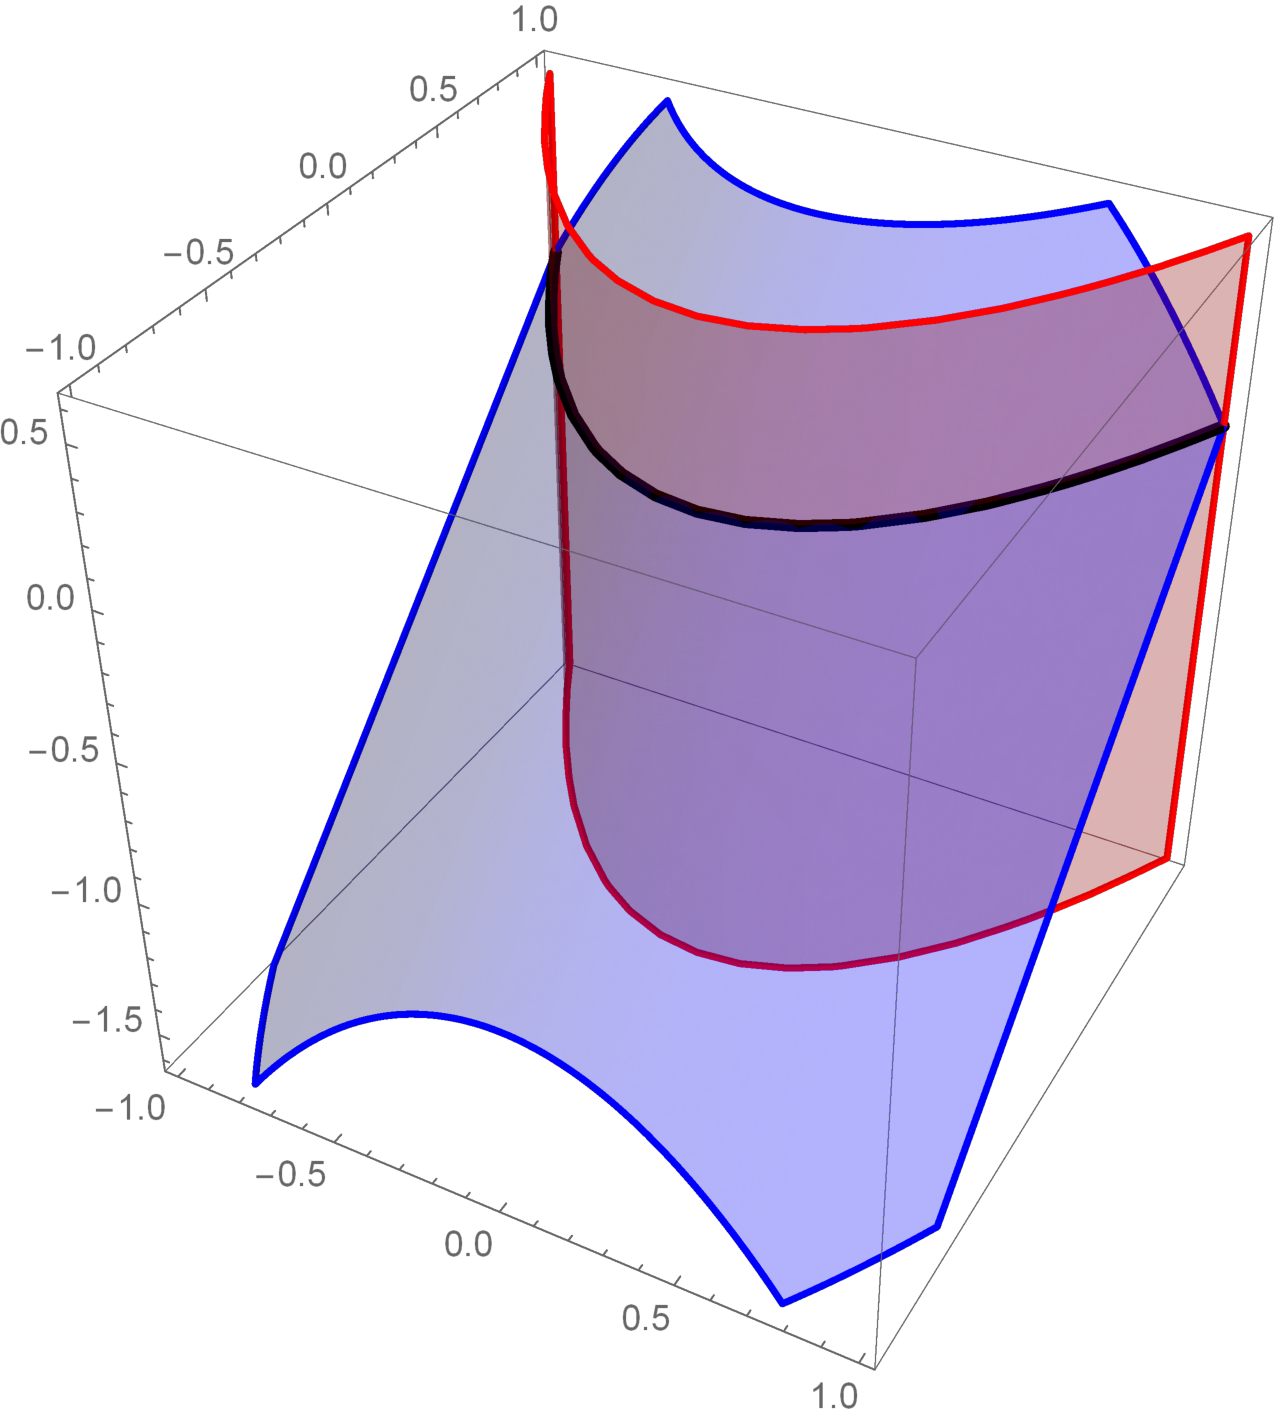
\includegraphics[scale=.5]{images/Together}
\end{figure}

\section{ParametricPlot}

Esse comando é bastante empregado como uma alternativa ao \ttt{Plot} ou \ttt{ContourPlot}. Com ele podemos fazer representações semelhantes, porém de forma mais simplificada e igualmente entendível. A primeira posição que passamos diz respeito a uma lista de parâmetros em $x$, $y$ e $z$, a depender se estamos tratando de duas ou três dimensões. 

Um exemplo clássico de ser tratado nessa etapa diz respeito à parametrização de uma circunferência, que nos remete à ideia de duas dimensões. Nesse exemplo, vamos fazer uso das coordenadas polares como forma de descrever a curva no plano. Dessa forma, da geometria analítica sabemos que as variáveis $x$ e $y$ assumem 

$$
\begin{cases}
	x=r\sin(t)\\
	y=r\cos(t)
\end{cases}
$$

Para a circunferência alvo de nosso estudo vamos imaginar que ela possui raio unitário, dessa forma teremos

$$
\begin{cases}
	x=\sin(t)\\
	y=\cos(t)
\end{cases}
$$

Para adequarmos à sintaxe do \ttt{ParametricPlot} mostrada abaixo

\begin{center}
	\ttt{ParametricPlot[\{$\ttt{f}_{\ttt{x}}$,$\ttt{f}_{\ttt{y}}$\},\{$\ttt{t}$,$\ttt{t}_{\ttt{mín}}$,$\ttt{t}_{\ttt{máx}}$\}]}
\end{center}

Vamos imaginar que a função que descreve o traçado da circunferência depende do tempo ($t$), assim quando $t=0$ a curva não começou a ser traçada, mas quando $t=\pi$, metade dela já foi renderizada. Com isso em mente, chegamos que quando $t=2\pi$ a representação da circunferência estará completa. Dessa forma, o \ttt{ParametricPlot} alcança a seguinte forma após assumirmos que $x$ e $y$ dependem de $t$

\begin{lstlisting}[language=Mathematica]
ParametricPlot[{Sin[t],Cos[t]},{t,0,2Pi}]
\end{lstlisting}

Podemos ler a linha acima como: ``Substitua $t$ no intervalo de 0 a $2\pi$ na função paramétrica de coordenadas $(\sin t,\cos t)$.''

\begin{figure}[!h]
	\centering
	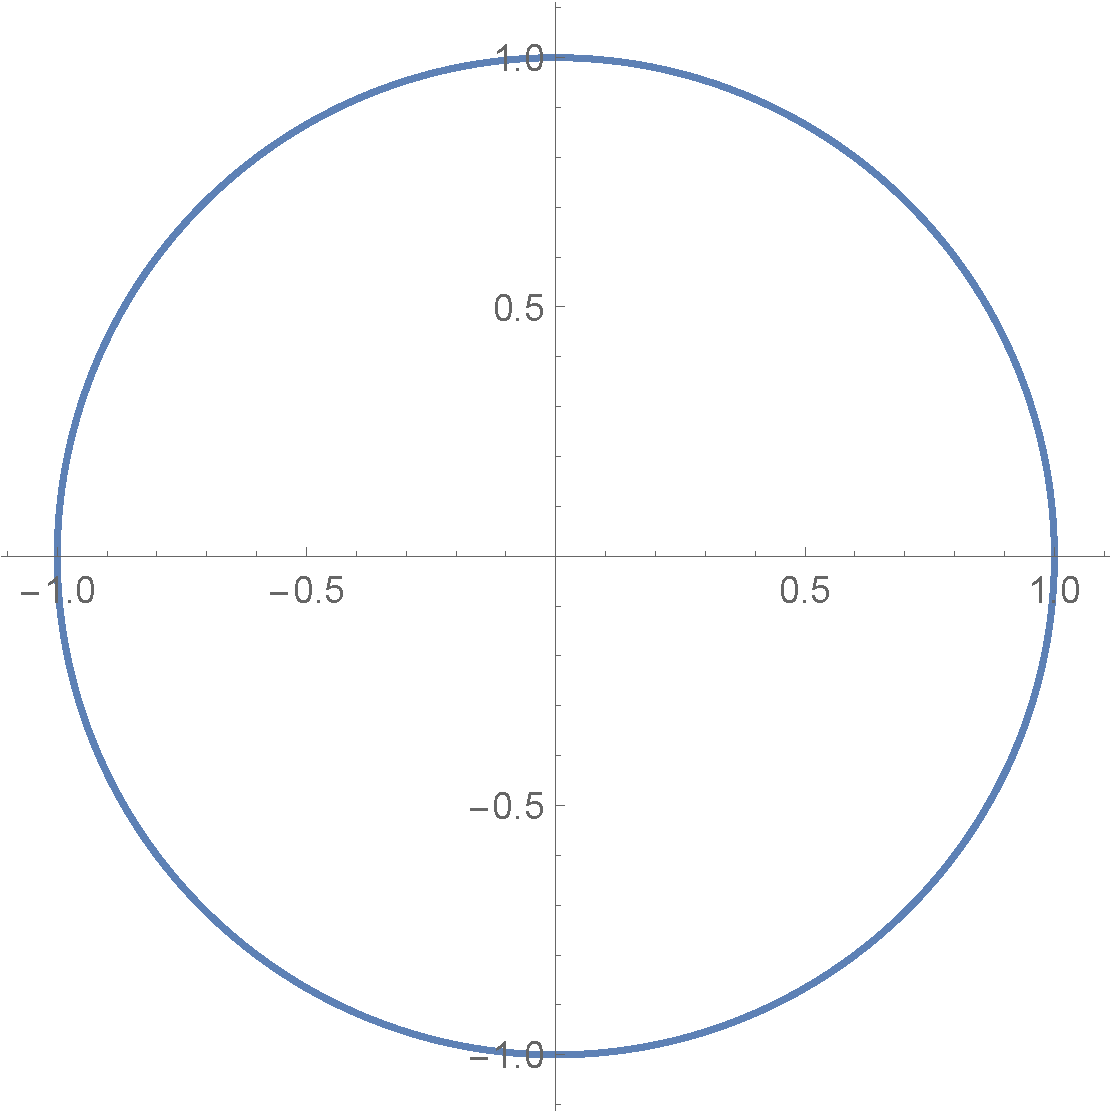
\includegraphics[scale=.5]{images/ParametricPlot}
\end{figure}

Repare que poderíamos assumir que $x=\cos(t)$ e $y=\sin(t)$ e isso só influenciaria no sentido da parametrização. Ou seja, ao invés de ser no sentido horário seria no anti-horário, mas o resultado final é o mesmo.

Para o \ttt{ParametricPlot3D} temos somente o acréscimo de uma nova posição na função paramétrica. Dessa forma, mudamos de \ttt{\{$\ttt{f}_{\ttt{x}}$,$\ttt{f}_{\ttt{y}}$\}} para \ttt{\{$\ttt{f}_{\ttt{x}}$,$\ttt{f}_{\ttt{y}}$,$\ttt{f}_{\ttt{z}}$\}}. Vamos usar um exemplo bastante análogo ao anterior, porém enquanto a circunferência é traçada em $x$ e $y$ vamos fazê-la ganhar altitude em $z$. Vejamos o exemplo

\begin{lstlisting}[language=Mathematica]
ParametricPlot3D[{Sin[t],Cos[t],t},{t,0,2Pi}]
\end{lstlisting}

\begin{figure}[!h]
	\centering
	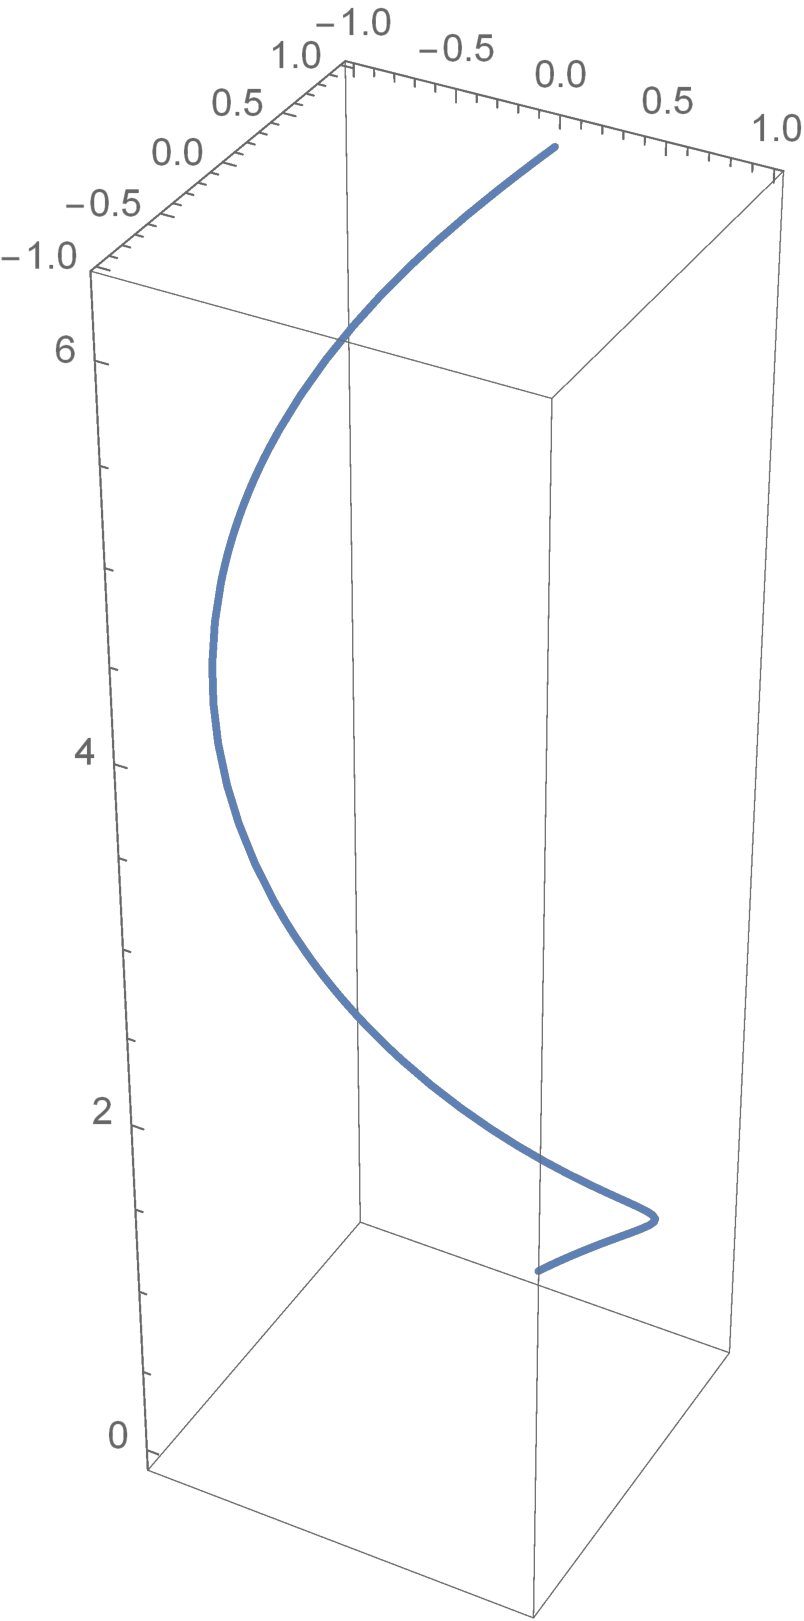
\includegraphics[scale=.5]{images/ParametricPlot3D}
\end{figure}

Mas o que houve nesse caso? Simples, ao adicionar o parâmetro t na na terceira posição da função paramétrica ocasionamos o deslocamento  dos pontos em $z$ como dito anteriormente. Dessa forma, vê-se que não só o ângulo $t$ vai de 0 a $2\pi$ nas funções $\sin$ e $\cos$, mas a altura do gráfico também. Isso ocasiona na cota 6 mostrada em $z$ (valor próximo dos 2$\pi\approx 6,\!28\ldots$) gerando a conformação de espiral mostrada. Como sabemos que $f_{x}$ e $f_{y}$ não foram modificadas se alterarmos a vista de \textit{Default} para \textit{Top}

\newpage
\begin{figure}[!h]
	\centering
	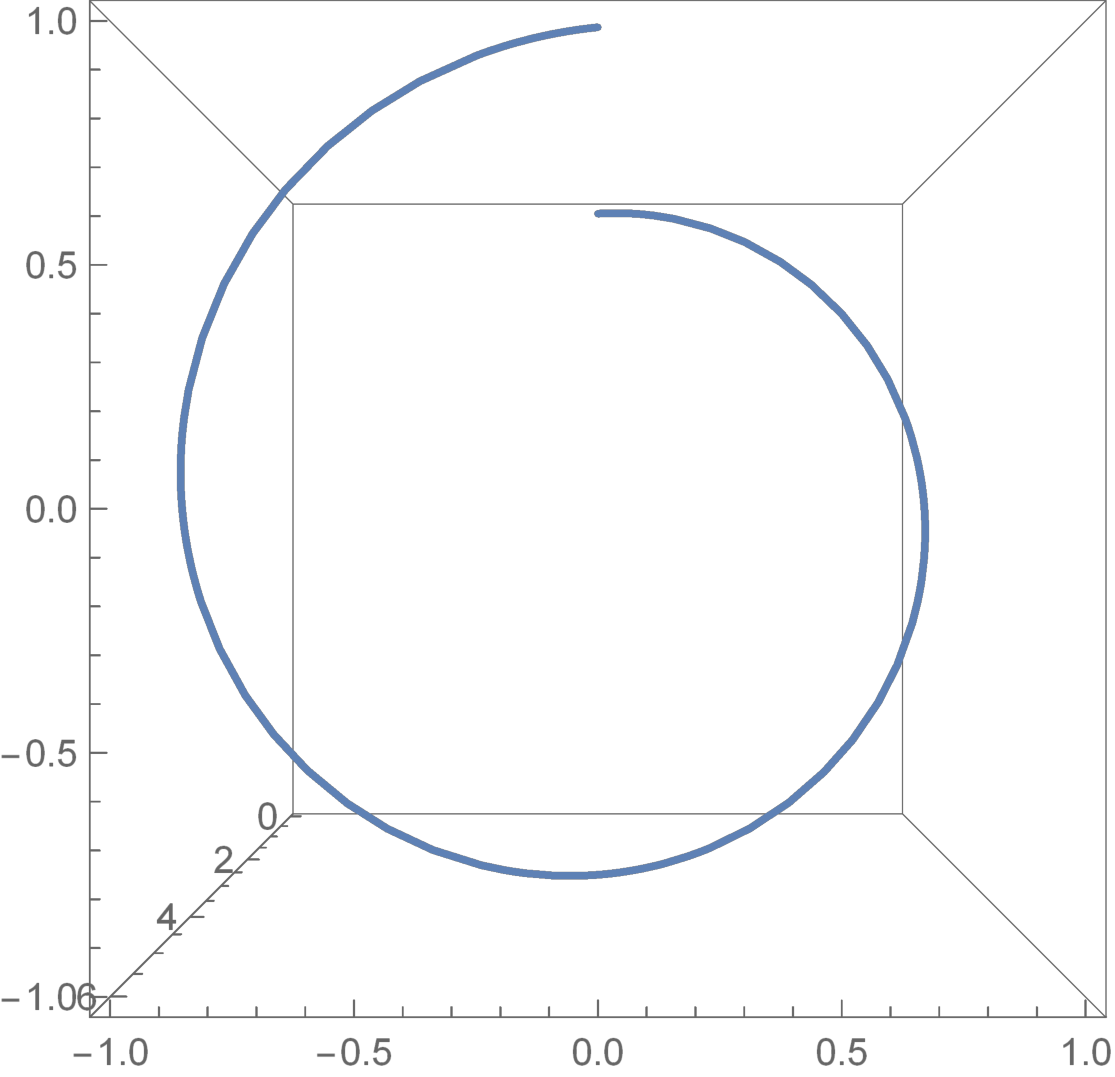
\includegraphics[scale=.5]{images/ParametricPlot3DTopView}
\end{figure}

veremos que a circunferência ainda existe na vista superior

Vamos supor agora que queremos mostrar dois pontos. Um estará no início da curva em espiral -- quando $t=0$ -- e outra ao final ($t=2\pi$). A ideia é simples, basta substituirmos esses valores de $t$ na função paramétrica e vamos obter

$$
\begin{cases}
	p_{1} = (\sin 0,\cos 0,0) \Rightarrow (0,1,0)\\
	p_{2} = (\sin 2\pi,\cos 2\pi, 2\pi) \Rightarrow (0,1,2\pi)
\end{cases}
$$

Para representarmos $p_{1}$ e $p_{2}$ graficamente vamos usar o comando \ttt{Graphics3D}. Como vamos plotar pontos, usamos o \ttt{Point} dentro dele da seguinte forma 

\begin{center}
	\ttt{Graphics3D[Point[]]}
\end{center}

Para aumentarmos o tamanho dos pontos na representação aplicamos o \ttt{PointSize}

\begin{center}
	\ttt{Graphics3D[\{PointSize[Large],Point[]\}]}
\end{center}

Podemos escolher as cores também. Vamos de \ttt{Magenta} nesse caso

\begin{center}
	\ttt{Graphics3D[\{PointSize[Large],Red,Point[]\}]}
\end{center}

Agora, dentro do \ttt{Point} basta acrescentarmos uma lista de pontos com a estrutura

\begin{center}
	\ttt{\{p1,p2,\ldots,$\ttt{p}_{\ttt{n}}$\}}
\end{center}

No nosso caso \ttt{p1\,=\,\{0,1,0\}} e \ttt{p2\,=\,\{0,1,2\,Pi\}}, assim o \ttt{ParametricPlot3D} assumirá a forma

\begin{center}
	\ttt{
		Graphics3D[\textcolor{purple}{\{}PointSize[Large],Point[\textcolor{red}{\{}\textcolor{blue}{\{0,1,0\},\{0,1,2\,Pi\}}\textcolor{red}{\}}]\textcolor{purple}{\}}]}
\end{center}

Escrevendo as seguintes linhas de código, obtemos

\begin{lstlisting}[language=Mathematica]
a = ParametricPlot3D[{Sin[t],Cos[t],t},{t,0,2Pi}]
b = Graphics3D[{PointSize[Large],Red,Point[{{0,1,0},{0,1,2Pi}}]}]
Show[a,b]
\end{lstlisting}

\begin{figure}[!h]
	\centering
	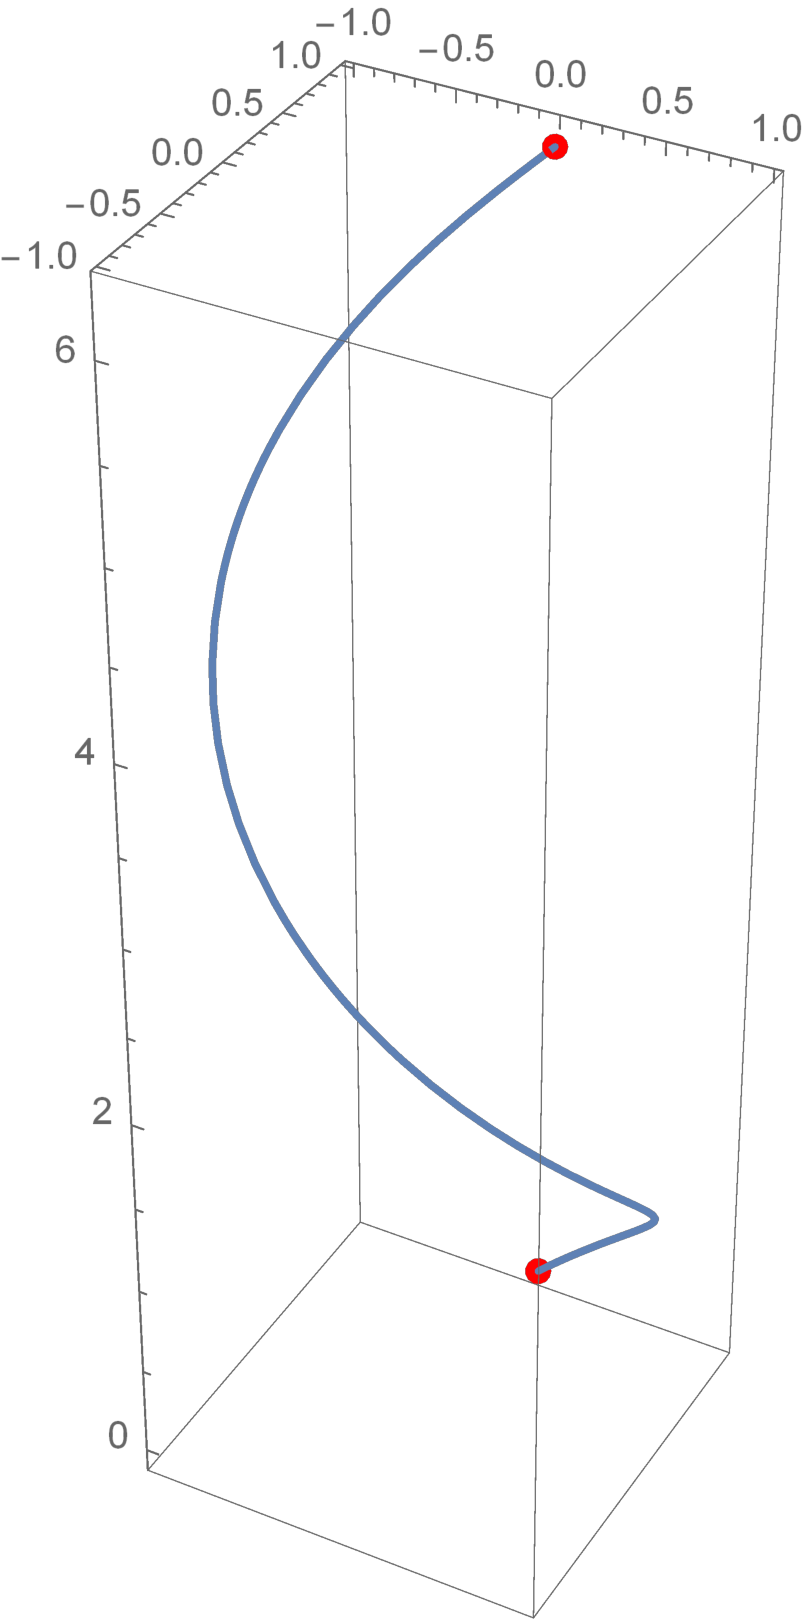
\includegraphics[scale=.24]{images/ShowParametricPlot}
\end{figure}


\newpage
Vamos acrescentar outro comando dentro do \ttt{Graphics} ainda não mostrado, o \ttt{Line}. A sintaxe é semelhante ao \ttt{Point}, nós passamos uma lista de pontos e, de forma automática, é feita a interligação entre eles com base na ordem em que são escritos dentro da lista. Como só serão passados dois pontos (\ttt{p1} e \ttt{p2}), ao digitar

\begin{lstlisting}[language=Mathematica]
c = Graphics3D[{PointSize[Large],Red,Thick,Line[{{0,1,0},{0,1,2Pi}}]}]
\end{lstlisting}

\begin{figure}[!h]
	\centering
	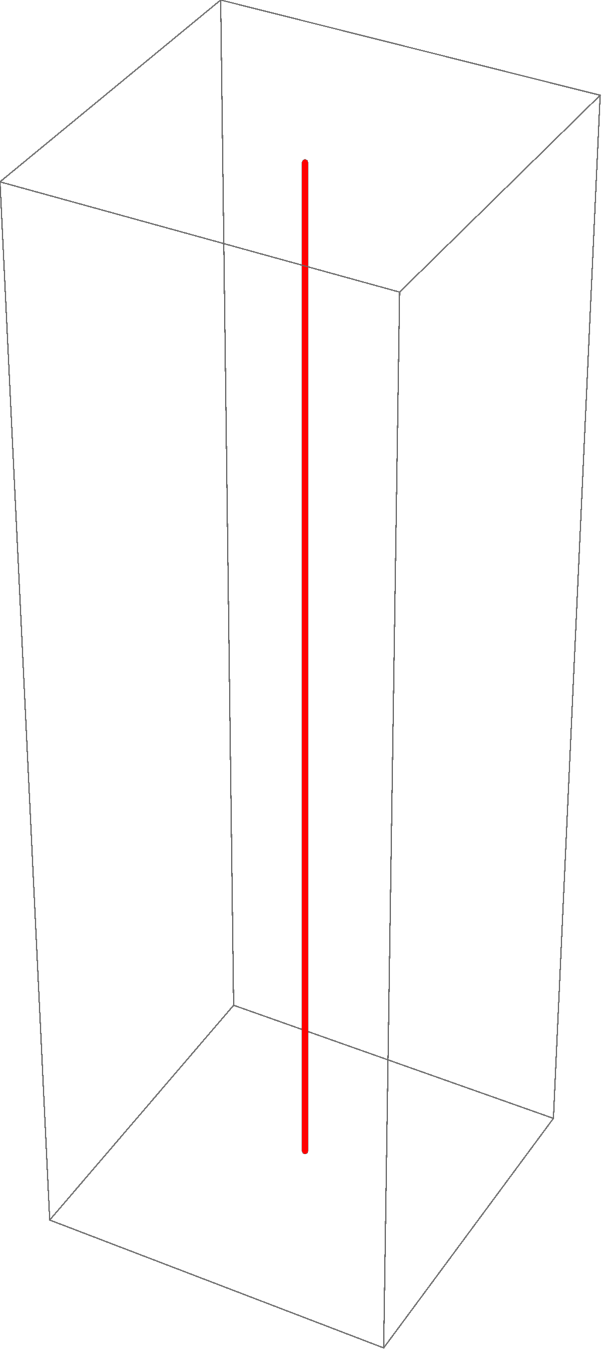
\includegraphics[scale=.3]{images/Line}
\end{figure}

Juntando \ttt{a}, \ttt{b} e \ttt{c} no \ttt{Show}

\begin{lstlisting}[language=Mathematica]
Show[a,b,c]
\end{lstlisting}

\begin{figure}[!h]
	\centering
	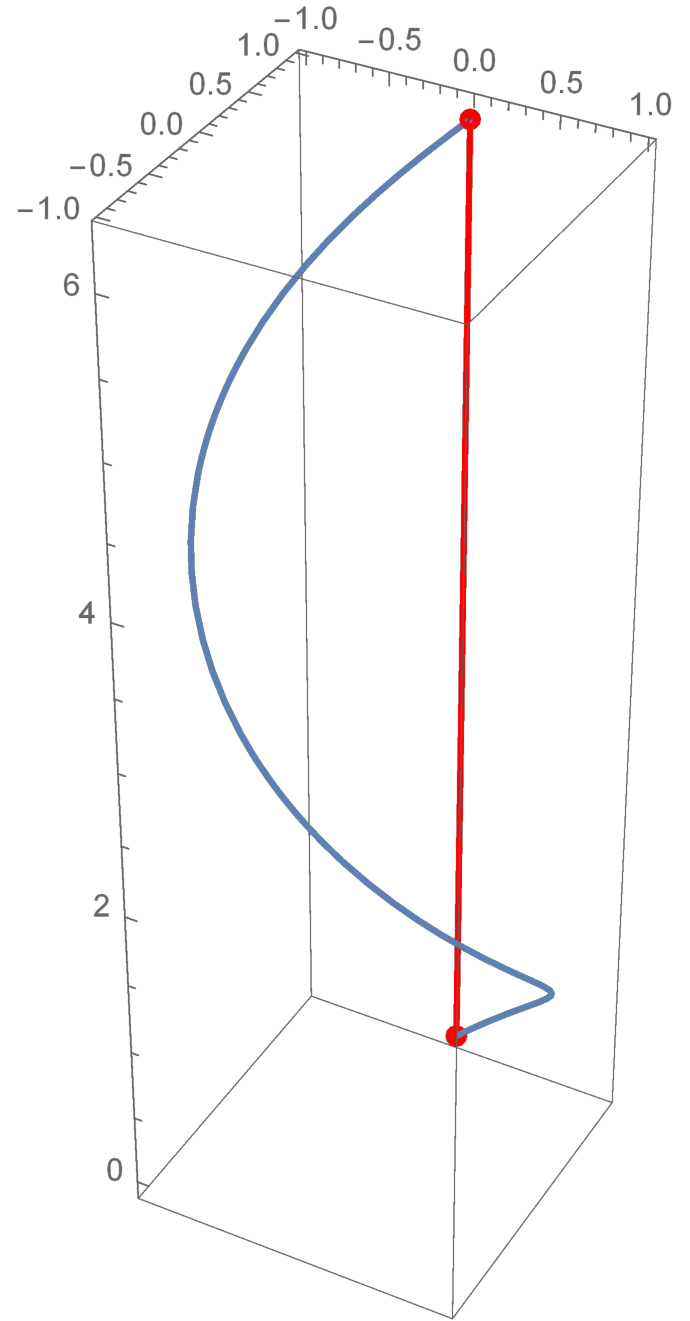
\includegraphics[scale=.5]{images/ShowNew}
\end{figure}

\newpage
\subsection{Outro exemplo com o ParametricPlot3D}

Vamos fazer um paraboloide análogo ao que foi feito com o \ttt{ContourPlot3D}. Basta estendermos a ideia do \ttt{ParametricPlot} para duas dimensões alterando a terceira posição da função ($f_{z}$). 

Imagine que o paraboloide é uma série de círculos superpostos de modo que o raio e altura de cada um deles no empilhamento dependam de $r$ e $t$. Nesse caso, $t$ terá o mesmo papel visto anteriormente: Fará o ângulo interno variar de 0 a $2\pi$, enquanto $r$ elevará a altura de cada circunferência e aumentará seu raio seguindo $r^{2}$.

Levando essa ideia para o \ttt{ParametricPlot3D}, podemos escrever

$$
\begin{cases}
	x=r\sin t\\
	y=r\cos t\\
	z=r^{2}
\end{cases}
$$

\begin{lstlisting}[language=Mathematica]
ParametricPlot3D[{r Sin[t],r Cos[t],r^2},{t,0,2Pi},{r,0,4}]
\end{lstlisting}

Podemos interpretar a linha acima como: ``A partir da variação de $t$, renderize várias circunferências com o raio e altura segundo $r$ (de 0 a 4 para o raio e de 0 a 16 para a altura)''
\end{document}
















